\documentclass[10pt,
  aspectratio=169,
  serif,
  mathserif,
  professionalfont,
  compress,
  handout,
  % table,
  % svgnames
  ]{beamer}\usepackage[]{graphicx}\usepackage[]{color}
% maxwidth is the original width if it is less than linewidth
% otherwise use linewidth (to make sure the graphics do not exceed the margin)
\makeatletter
\def\maxwidth{ %
  \ifdim\Gin@nat@width>\linewidth
    \linewidth
  \else
    \Gin@nat@width
  \fi
}
\makeatother

\definecolor{fgcolor}{rgb}{1, 1, 0.941}
\newcommand{\hlnum}[1]{\textcolor[rgb]{0.804,0.718,0.71}{#1}}%
\newcommand{\hlstr}[1]{\textcolor[rgb]{0.604,0.753,0.804}{#1}}%
\newcommand{\hlcom}[1]{\textcolor[rgb]{0.439,0.502,0.565}{#1}}%
\newcommand{\hlopt}[1]{\textcolor[rgb]{1,1,0.941}{#1}}%
\newcommand{\hlstd}[1]{\textcolor[rgb]{1,1,0.941}{#1}}%
\newcommand{\hlkwa}[1]{\textcolor[rgb]{0.941,0.902,0.549}{#1}}%
\newcommand{\hlkwb}[1]{\textcolor[rgb]{1,0.871,0.678}{#1}}%
\newcommand{\hlkwc}[1]{\textcolor[rgb]{0.545,0.941,0.702}{#1}}%
\newcommand{\hlkwd}[1]{\textcolor[rgb]{0.545,0.941,0.902}{#1}}%
\let\hlipl\hlkwb

\usepackage{framed}
\makeatletter
\newenvironment{kframe}{%
 \def\at@end@of@kframe{}%
 \ifinner\ifhmode%
  \def\at@end@of@kframe{\end{minipage}}%
  \begin{minipage}{\columnwidth}%
 \fi\fi%
 \def\FrameCommand##1{\hskip\@totalleftmargin \hskip-\fboxsep
 \colorbox{shadecolor}{##1}\hskip-\fboxsep
     % There is no \\@totalrightmargin, so:
     \hskip-\linewidth \hskip-\@totalleftmargin \hskip\columnwidth}%
 \MakeFramed {\advance\hsize-\width
   \@totalleftmargin\z@ \linewidth\hsize
   \@setminipage}}%
 {\par\unskip\endMakeFramed%
 \at@end@of@kframe}
\makeatother

\definecolor{shadecolor}{rgb}{.97, .97, .97}
\definecolor{messagecolor}{rgb}{0, 0, 0}
\definecolor{warningcolor}{rgb}{1, 0, 1}
\definecolor{errorcolor}{rgb}{1, 0, 0}
\newenvironment{knitrout}{}{} % an empty environment to be redefined in TeX

\usepackage{alltt}

% Tamanho de fonte e distância entre linhas.
\renewenvironment{knitrout}{
  \renewcommand{\baselinestretch}{0.75}%\tiny
}{}

%-----------------------------------------------------------------------
% Pacotes padrões.

% Fontes.
\usepackage{palatino}
\usepackage{eulervm}
\usepackage{inconsolata}

% Esses pacotes dão clash.
% http://tex.stackexchange.com/questions/51488/option-clash-with-xcolor-and-tikz
% \usepackage{xcolor} %% opções no \documentclass{} para evitar clash.
% \definecolor{mycolor}{rgb}{0.13,0.53,0.53}
% \definecolor{mycolor2}{rgb}{0.725,0,0.18}

\usepackage{hyperref}
 \hypersetup{colorlinks, allcolors=., urlcolor=structure}
% \hypersetup{colorlinks}

\usepackage[brazil]{babel}
\usepackage[utf8]{inputenc}
\usepackage{graphicx}
\usepackage{amsmath, amsfonts, amssymb, amsxtra, amsthm, icomma}
\usepackage{geometry, calc, setspace, indentfirst}
% \usepackage{colortbl}
\usepackage{enumerate}
\usepackage{float}

\usepackage{subfigure}

\usepackage[hang]{caption}
\captionsetup{font=footnotesize,
  labelfont=footnotesize,
  labelsep=period}

% Listas em duas colulas.
\usepackage{multicol}
\newenvironment{itemize2}{%
  \vspace*{-1em}
  \begin{itemize}
    \begin{multicols}{2}
    }{%
    \end{multicols}
  \end{itemize}
}

% Texto no corpo do beamer justificado.
\usepackage{ragged2e}
\justifying

%-----------------------------------------------------------------------

% A lot of options:
% http://latex-community.org/forum/viewtopic.php?f=55&t=17646
\useoutertheme[
  width=60pt,
  height=30pt,
  right,
  hideothersubsections
  ]{sidebar}

\makeatletter
\setbeamertemplate{caption}[numbered]
\setbeamertemplate{section in toc}[sections numbered]
\setbeamertemplate{subsection in toc}[subsections numbered]
\setbeamertemplate{sections/subsections in toc}[ball]{}
\setbeamertemplate{section in sidebar right}[sections numbered]
%\setbeamertemplate{frametitle continuation}{\gdef\beamer@frametitle{}}
\setbeamertemplate{navigation symbols}{} %% Retira a barra de navegação.
% \setbeamertemplate{blocks}[rounded][shadow=FALSE]
% \setbeamercolor{block title}{fg=structure, bg=mycolor!20!white}
\makeatother

% Frames com sessão e/ou subsessão.
% \addtobeamertemplate{frametitle}{
%   \let\insertframetitle\insertsubsectionhead}{}
% \makeatletter
% \CheckCommand*\beamer@checkframetitle{
%   \@ifnextchar\bgroup\beamer@inlineframetitle{}}
% \renewcommand*\beamer@checkframetitle{
%   \global\let\beamer@frametitle\relax\@ifnextchar\bgroup
%   \beamer@inlineframetitle{}}
% \makeatother

\setbeamertemplate{frametitle}
{
    \nointerlineskip
    \begin{beamercolorbox}[sep=0.3cm,ht=1.8em,wd=\paperwidth]{frametitle}
        \vbox{}\vskip-2ex%
        \strut\insertframetitle\strut
        \vskip-0.8ex%
    \end{beamercolorbox}
}

%-----------------------------------------------------------------------
% Comandos.

\newcommand{\n}[1]{\textbf{#1}}

%-----------------------------------------------------------------------

\AtBeginSection[]{
  \begin{frame}[c,allowframebreaks]
    \begin{center}
      {\thesection} \\ \vspace{0.3cm}
      \parbox{0.6\textwidth}{
        \centering {\Large \textcolor{structure}{\insertsection}}}\\
    \end{center}
  \end{frame}
}

%-----------------------------------------------------------------------
% Definições dos proprietários.

\title[Aula Inaugural]{
  \LARGE Experiências do curso de\\ graduação em Estatística \vspace{0.2cm}}


\subtitle{Aula inaugural 2021}


\author[Lineu Alberto]{%\small
  Lineu Alberto Cavazani de Freitas \\
  \href{}{https://lineu96.github.io/st/}
}

\institute[UFPR]{}

\date{}

\logo{
\includegraphics[width=1.5cm]{img/dsbd1x4-rect.png}} 

\usebackgroundtemplate{
  
\includegraphics[width=\paperwidth]{img/ufpr-fundo.jpg}
}



\titlegraphic{
  \vspace{-1em}
  
\includegraphics[height=1.8cm]{img/ufpr-transparent.png}
}

%=======================================================================
%=======================================================================
\IfFileExists{upquote.sty}{\usepackage{upquote}}{}
\begin{document}

\frame{
  \titlepage
}

% Tabela de conteúdo no início dos slides.
 % \begin{frame}{Conteúdo}
 %   \small{\tableofcontents}
 % \end{frame}

%-----------------------------------------------------------------------



% -----------------------------------------------------------------

\section{Quem sou eu}

\begin{frame}
\frametitle{Quem sou eu}
\begin{columns}
\begin{column}{0.7\textwidth}
   \begin{itemize}

  \item Estatístico formado pela \href{https://www.ufpr.br/portalufpr/}{Universidade Federal do Paraná (UFPR)} em 2019.

  \item Atualmente mestrando no \href{http://www.prppg.ufpr.br/ppginformatica/?lang=pb}{Programa de Pós Graduação em Informática da UFPR}.

  \item Inserido na área de concentração Ciência da Computação, linha de pesquisa Tecnologia da Informação e grupo de pesquisa \href{https://web.inf.ufpr.br/dsbd/}{Data Science \& Big Data}.
  
  \end{itemize}
  
\end{column}
\begin{column}{0.3\textwidth}  %%<--- here
    \begin{center}
     
\includegraphics[width=\textwidth]{img/eu3.jpeg}
     \end{center}
\end{column}
\end{columns}
\end{frame}

% -----------------------------------------------------------------

\section{Minha trajetória na UFPR}

\begin{frame}

\begin{center}
  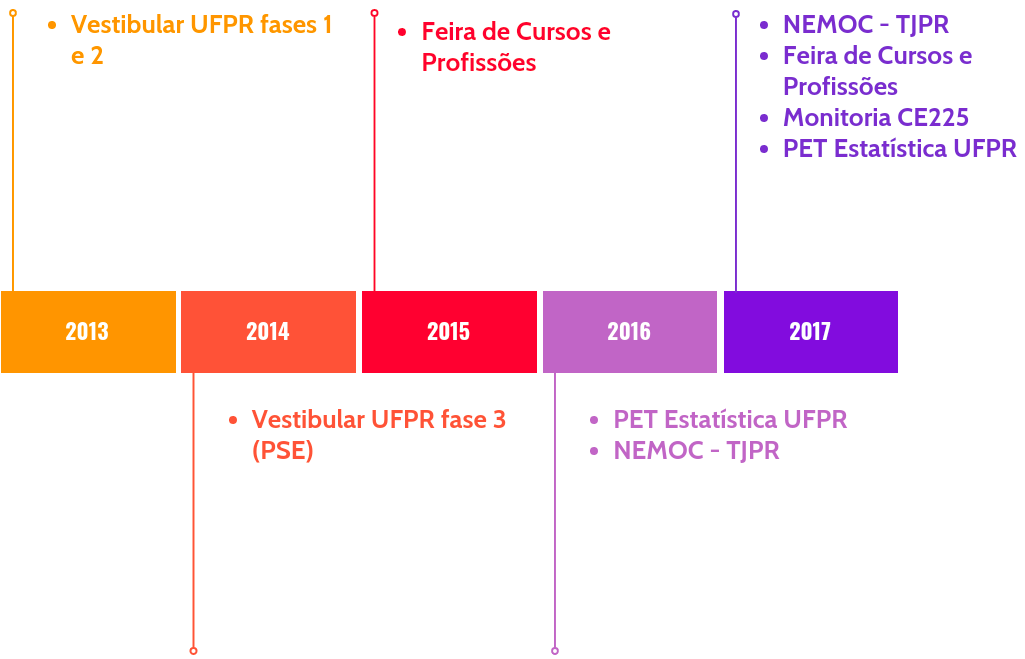
\includegraphics[width=11.7cm]{img/timeline11.png}
\end{center}

\end{frame}

% -----------------------------------------------------------------

\begin{frame}

\begin{center}
  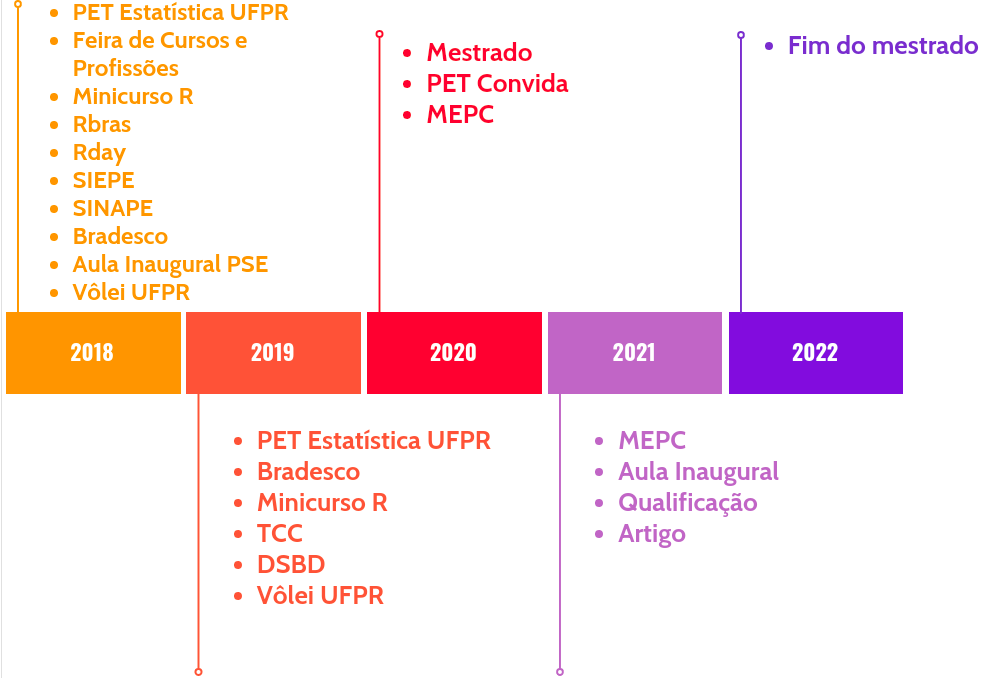
\includegraphics[width=10.98cm]{img/timeline12.png}
\end{center}

\end{frame}

% -----------------------------------------------------------------

\subsection{2013/14}

\begin{frame}[c, allowframebreaks]

\begin{center}

  {\huge \href{https://lineu96.github.io/st/}{2013/14}}
  
\end{center}

\end{frame}

%-----------------------------------------------------------------------

\begin{frame}

\frametitle{Vestibular UFPR - primeira fase}

\begin{center}
  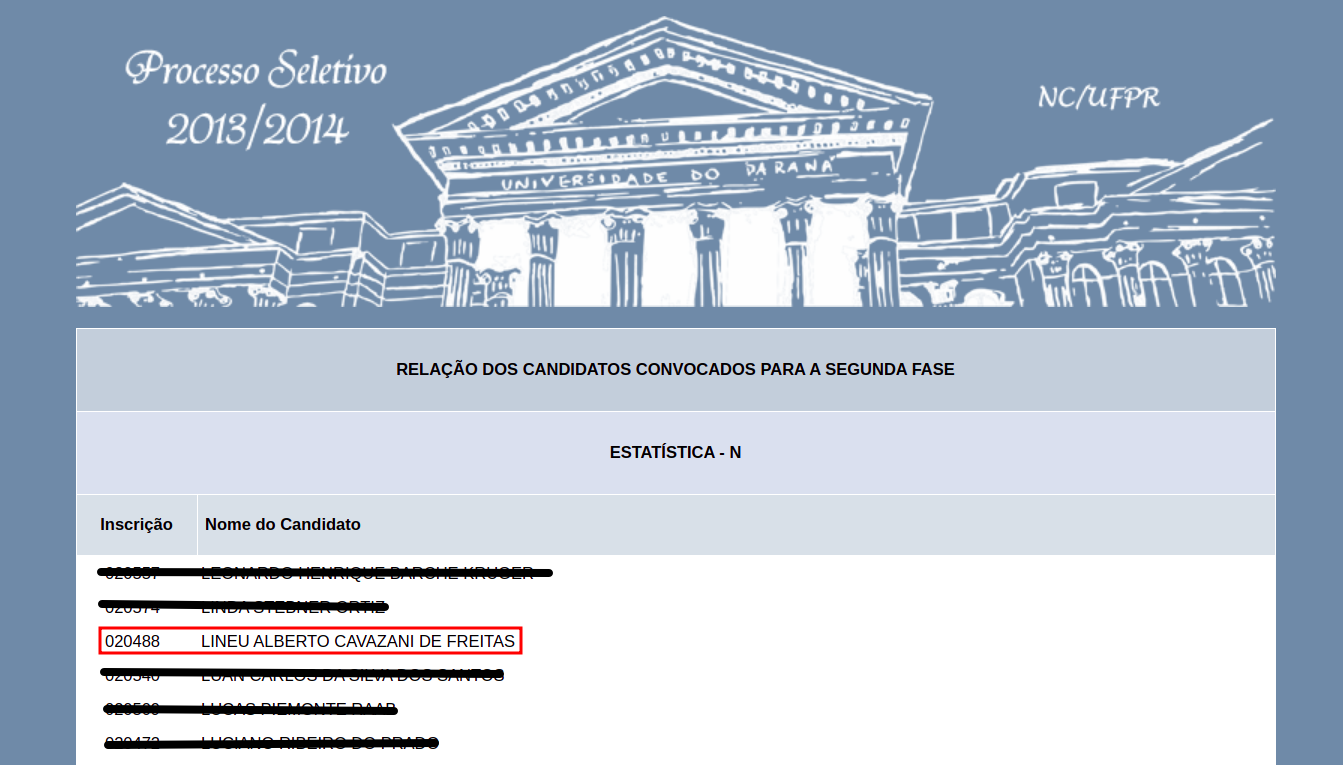
\includegraphics[width=11cm]{img/fase1.png}
\end{center}

\end{frame}

% -----------------------------------------------------------------

\begin{frame}

\frametitle{Vestibular UFPR - segunda fase}

\begin{center}
  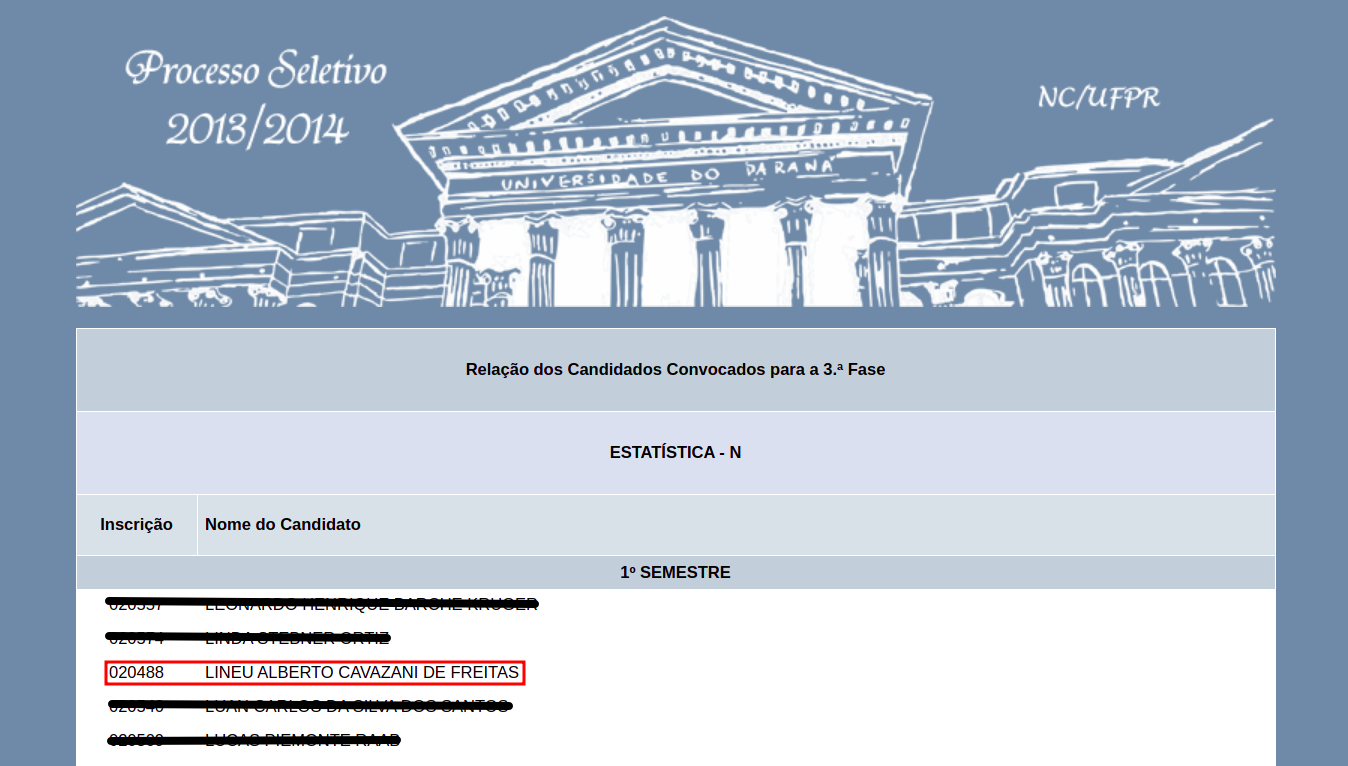
\includegraphics[width=11cm]{img/fase2.png}
\end{center}

\end{frame}

% -----------------------------------------------------------------

\begin{frame}

\frametitle{Vestibular UFPR - terceira fase}

\begin{center}
  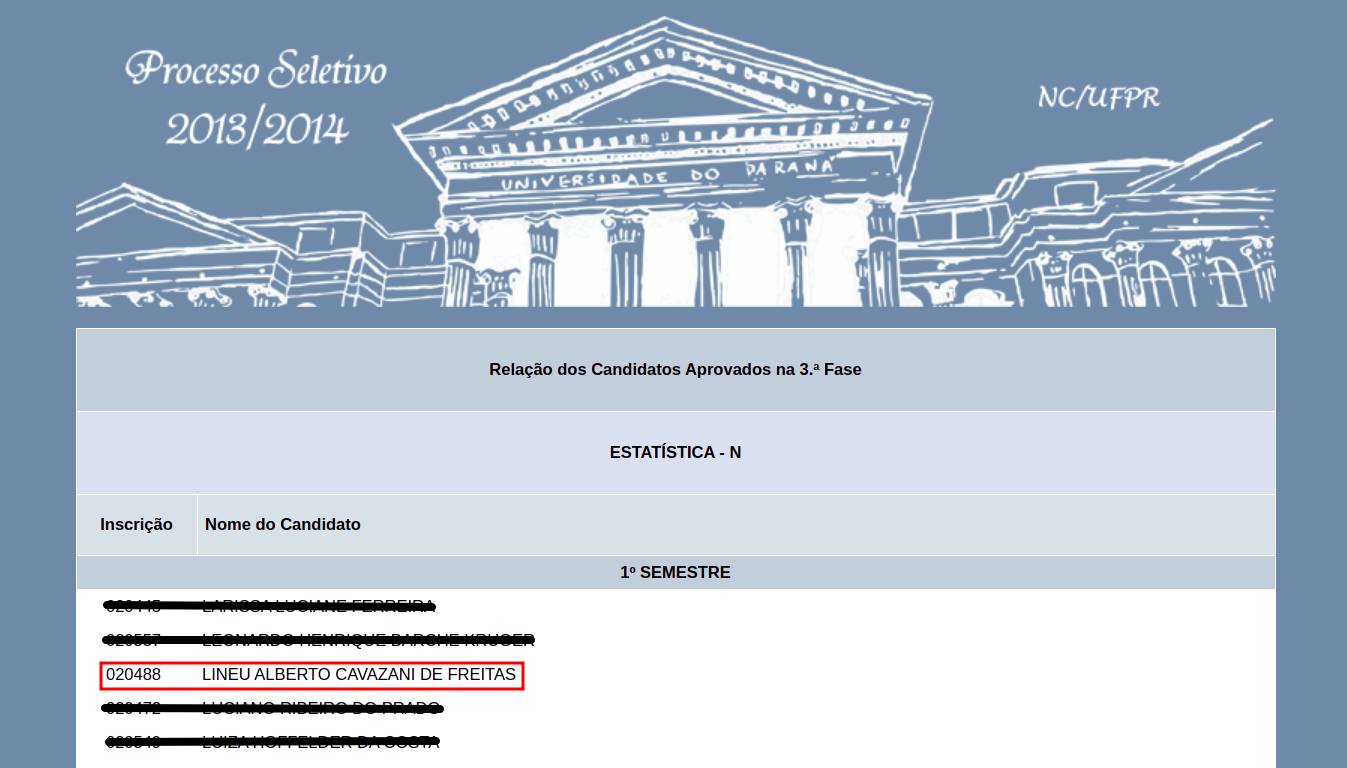
\includegraphics[width=11cm]{img/fase3.png}
\end{center}

\end{frame}

% -----------------------------------------------------------------

\subsection{2015}

\begin{frame}[c, allowframebreaks]

\begin{center}

  {\huge \href{https://lineu96.github.io/st/}{2015}}
  
\end{center}

\end{frame}

%-----------------------------------------------------------------------

\begin{frame}

\frametitle{Feira de cursos e profissões 2015}

\begin{center}
  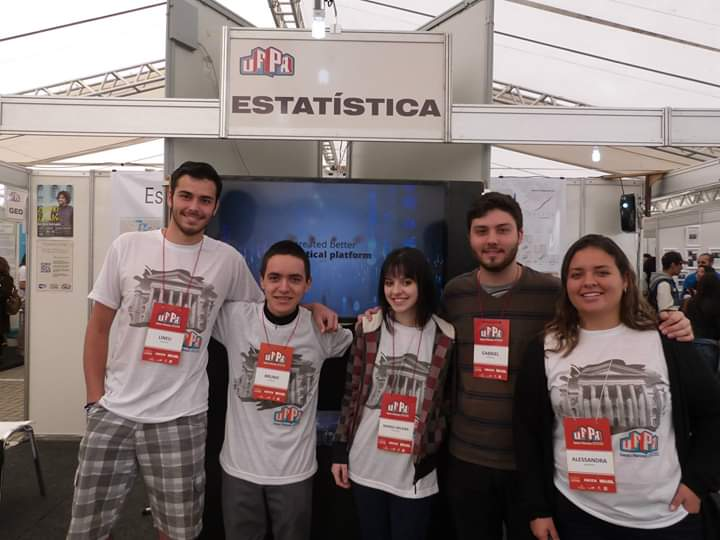
\includegraphics[width=8cm]{img/feira1.jpg}
\end{center}

\end{frame}

%-----------------------------------------------------------------------

\begin{frame}

\frametitle{Feira de cursos e profissões 2015}

\begin{center}
  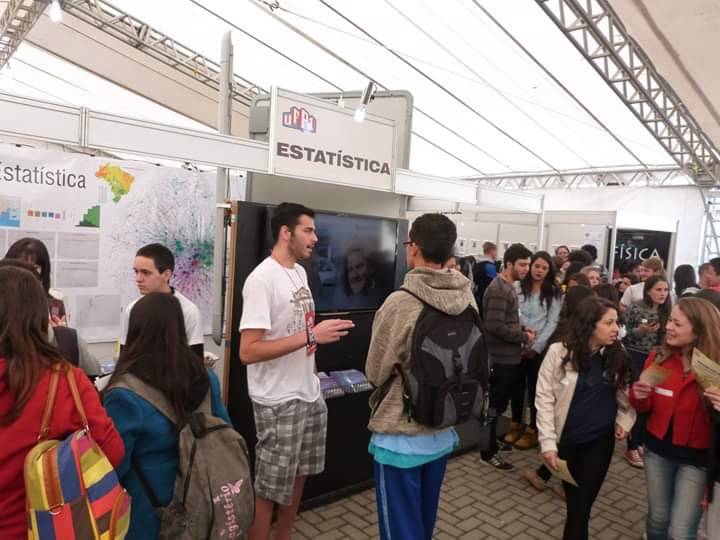
\includegraphics[width=8cm]{img/feira2.jpg}
\end{center}

\end{frame}

%-----------------------------------------------------------------------

\subsection{2016}

\begin{frame}[c, allowframebreaks]

\begin{center}

  {\huge \href{https://lineu96.github.io/st/}{2016}}
  
\end{center}

\end{frame}

%-----------------------------------------------------------------------

\begin{frame}

\frametitle{2016}

\begin{itemize}
  \item 1 semestre de Programa de Educação Tutorial
\end{itemize}

\begin{center}
  
\includegraphics[height=1.8cm]{img/pet.png}
\end{center}

\begin{itemize}
  \item NEMOC-TJPR
\end{itemize}

\begin{center}
  
\includegraphics[height=1.8cm]{img/tjpr.png}\hspace{2em}
  
\includegraphics[height=1.8cm]{img/corregedoria.png}\hspace{2em}
  
\includegraphics[height=1.8cm]{img/nemoc.png}
\end{center}

\end{frame}

% -----------------------------------------------------------------

\subsection{2017}

\begin{frame}[c, allowframebreaks]

\begin{center}

  {\huge \href{https://lineu96.github.io/st/}{2017}}
  
\end{center}

\end{frame}

% -----------------------------------------------------------------

\begin{frame}

\frametitle{Saída do NEMOC}

\begin{center}
  
\includegraphics[height=1.8cm]{img/tjpr.png}\hspace{2em}
  
\includegraphics[height=1.8cm]{img/corregedoria.png}\hspace{2em}
  
\includegraphics[height=1.8cm]{img/nemoc.png}
\end{center}

\end{frame}

% -----------------------------------------------------------------

\begin{frame}

\frametitle{Monitoria CE225}

\begin{center}
  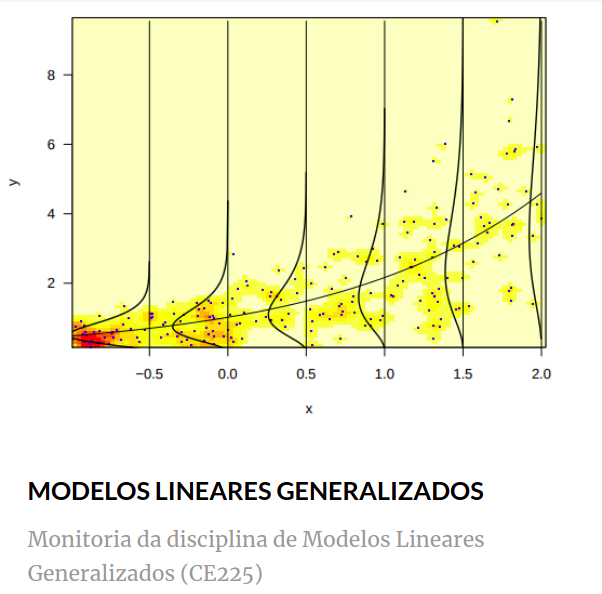
\includegraphics[height=6.5cm]{img/monitoria1.png}
\end{center}

\end{frame}

% -----------------------------------------------------------------

\begin{frame}

%\frametitle{Monitoria CE225}

\begin{center}
  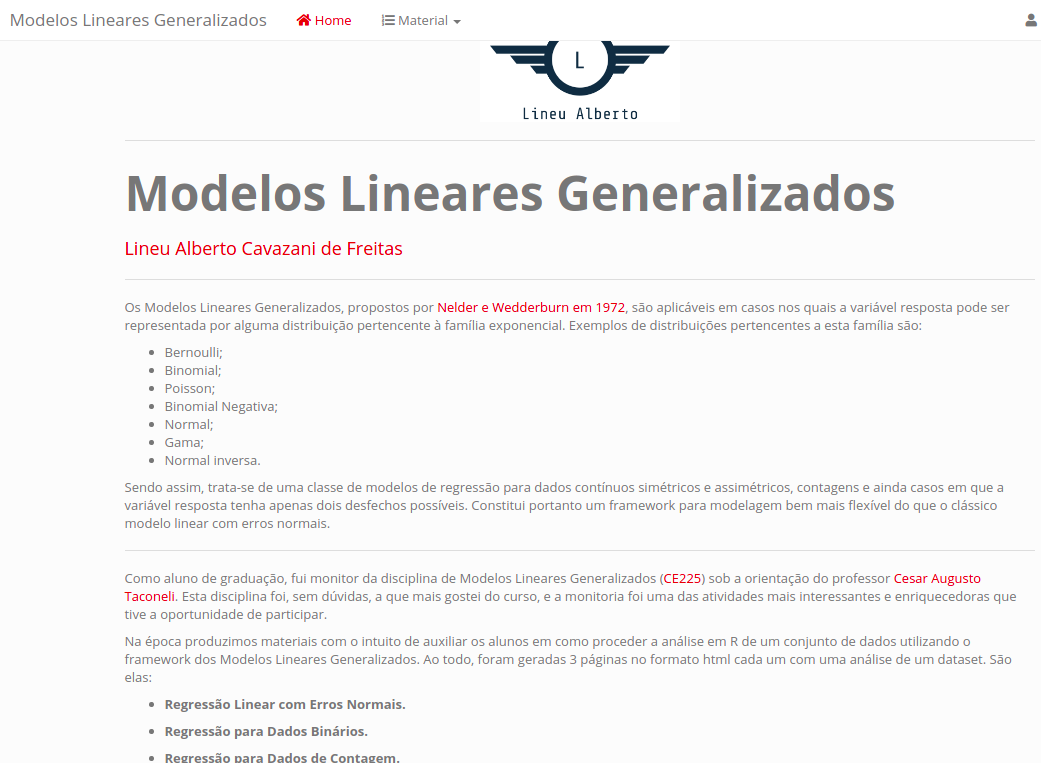
\includegraphics[height=7.5cm]{img/glm.png}
\end{center}

\end{frame}

% -----------------------------------------------------------------

\begin{frame}

\frametitle{Análise comportamental de ovelhas submetidas a intervenção humana}

\begin{center}
  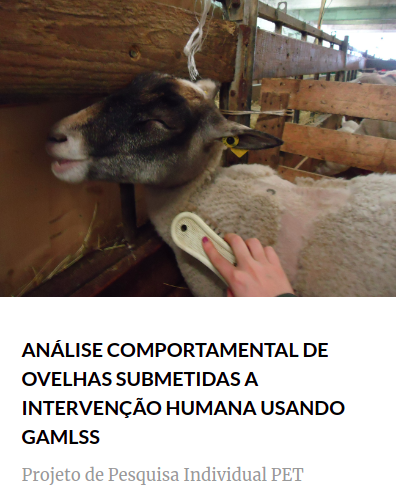
\includegraphics[height=6cm]{img/gamlss.png}
\end{center}

\end{frame}

% -----------------------------------------------------------------

\begin{frame}

\frametitle{Programa de Educação Tutorial}

\begin{center}
  
\includegraphics[height=3cm]{img/pet.png}
\end{center}

\end{frame}

% -----------------------------------------------------------------

\begin{frame}

\frametitle{Feira de cursos e profissões 2017}

\begin{columns}

\begin{column}{0.7\textwidth}

\begin{center}
     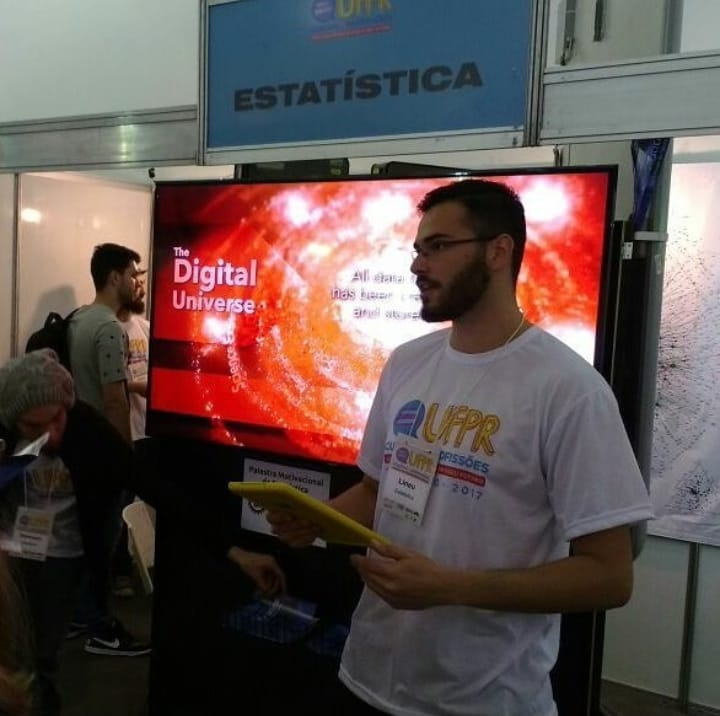
\includegraphics[width=6cm]{img/feira3.jpeg}
     \end{center}
  
\end{column}

\begin{column}{0.3\textwidth}  %%<--- here

    \begin{center}
     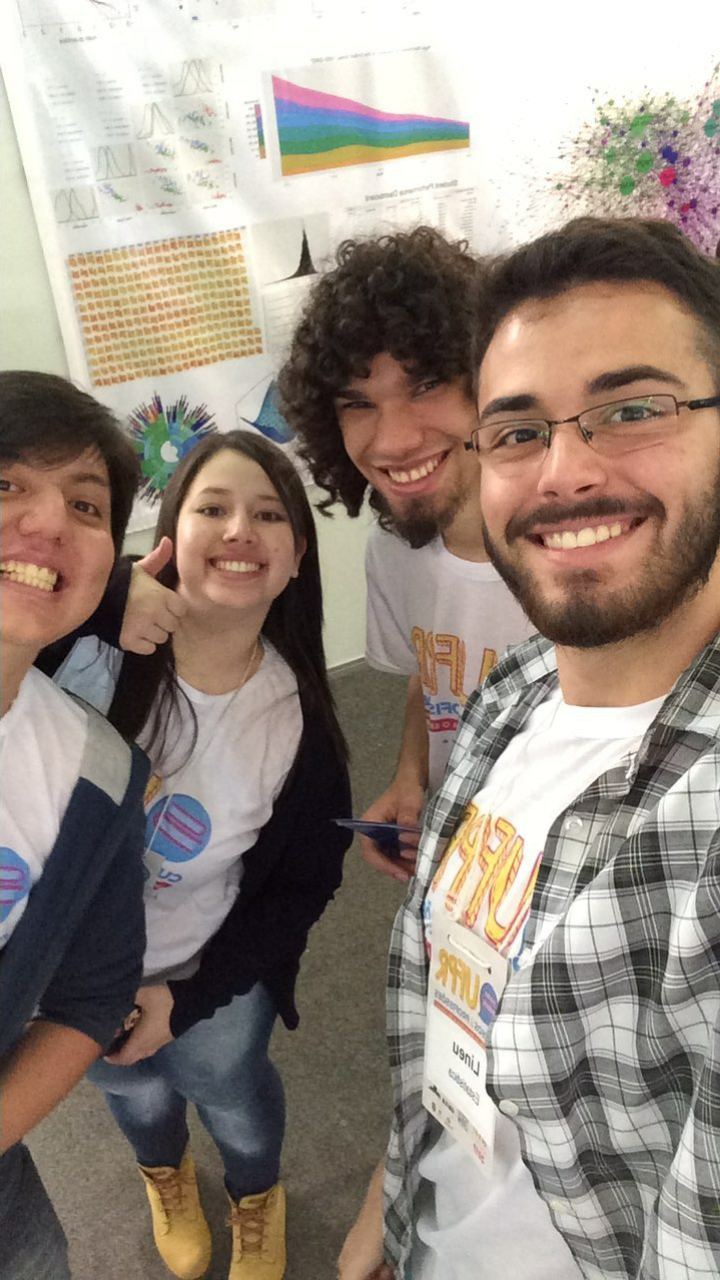
\includegraphics[width=3.4cm]{img/feira4.png}
     \end{center}

\end{column}

\end{columns}

\end{frame}

% -----------------------------------------------------------------

\subsection{2018}

\begin{frame}[c, allowframebreaks]

\begin{center}

  {\huge \href{https://lineu96.github.io/st/}{2018}}
  
\end{center}

\end{frame}

%-----------------------------------------------------------------------

\begin{frame}

\frametitle{Programa de Educação Tutorial}

\begin{center}
  
\includegraphics[height=3cm]{img/pet.png}
\end{center}

\end{frame}

% -----------------------------------------------------------------

\begin{frame}

\frametitle{Feira de Cursos e Profissões 2018}

\begin{center}
  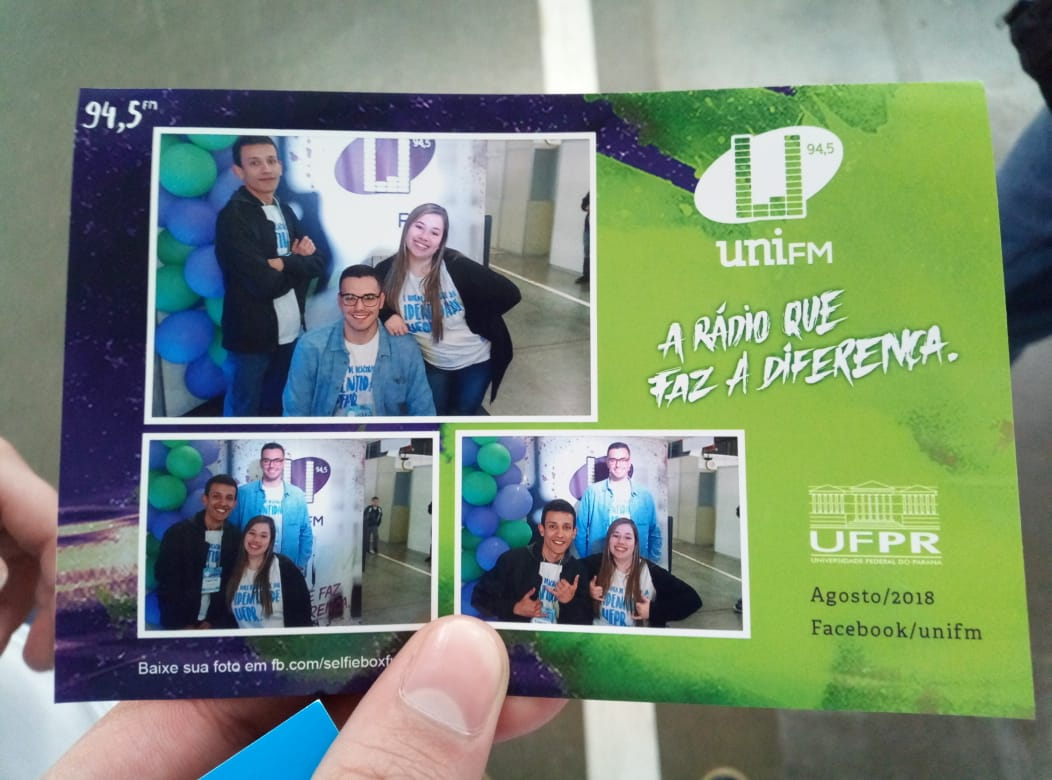
\includegraphics[height=6.5cm]{img/feira5.jpg}
\end{center}

\end{frame}

% -----------------------------------------------------------------

\begin{frame}

\frametitle{Minicurso R}

\begin{center}
  
\includegraphics[height=4cm]{img/minicurso1.png}
\end{center}

\end{frame}

% -----------------------------------------------------------------

\begin{frame}

\frametitle{Rbras 63 \& Rday}

\begin{center}
  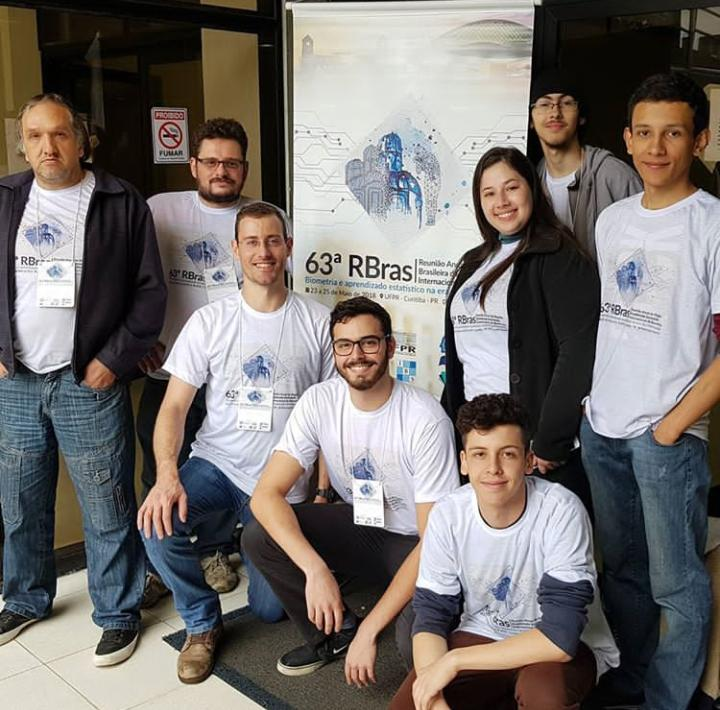
\includegraphics[height=6.5cm]{img/rbras.jpg}
\end{center}

\end{frame}


% -----------------------------------------------------------------

\begin{frame}
  \frametitle{Análise comportamental de ovelhas submetidas a intervenção humana}
  \begin{itemize}
    \itemsep 2ex
  
  \item Projeto de pesquisa desenvolvido no PET Estatística - UFPR sob orientação dos professores Cesar Augusto Taconeli e José Luiz Padilha da Silva. 
  
  \item Trabalho dividido em 3 etapas:
  
  \begin{enumerate}
    \itemsep 2ex
    
    \item A primeira parte foi apresentada na sessão pôster da 63ª Reunião Anual da Região Brasileira da Sociedade Internacional de Biometria (RBras).
    
    \item A segunda foi apresentada na sessão pôster do 23º Simpósio Nacional de Probabilidade e Estatística (SINAPE).
    
    \item O trabalho completo foi apresentado no 17º Encontro das Atividades Formativas (ENAF), evento componente da 10ª Semana Integrada de Ensino, Pesquisa e Extensão (SIEPE), como comunicação oral.
    
  \end{enumerate}
  
  \end{itemize}
\end{frame}

% -----------------------------------------------------------------

\begin{frame}

\frametitle{Análise comportamental de ovelhas submetidas a intervenção humana}

\begin{center}
  \includegraphics[height=6.5cm]{img/escov.png}
\end{center}

\end{frame}

% -----------------------------------------------------------------

\begin{frame}

\frametitle{Rbras}

\begin{center}
  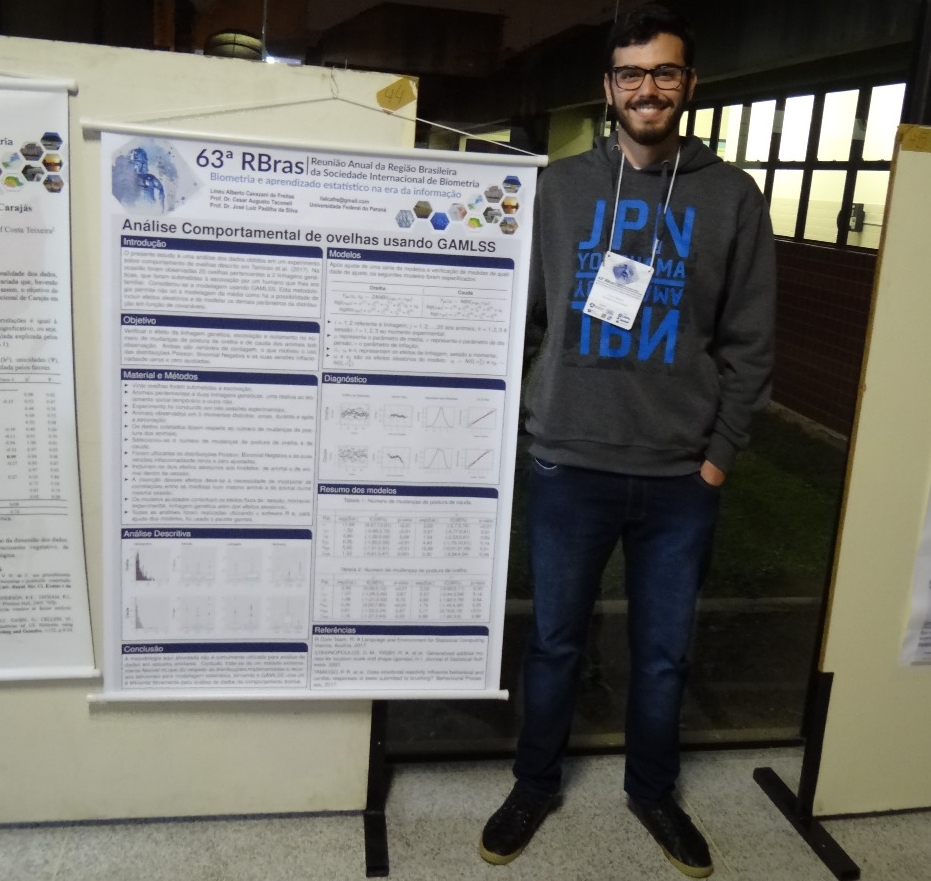
\includegraphics[height=6.5cm]{img/rbras3.jpg}
\end{center}

\end{frame}

% -----------------------------------------------------------------

\begin{frame}

\frametitle{Rbras}

\begin{center}
  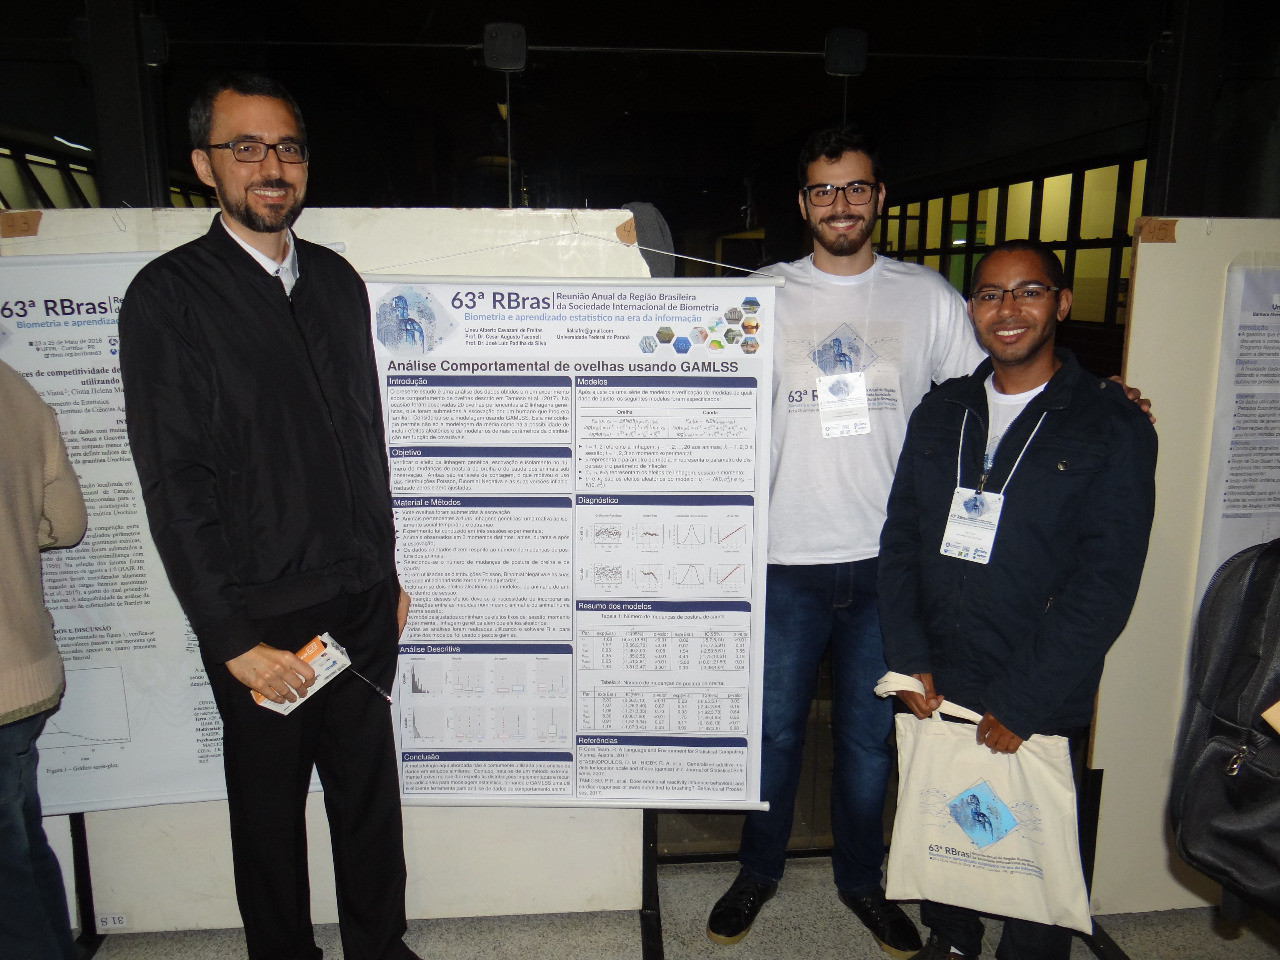
\includegraphics[height=6.5cm]{img/rbras2.jpg}
\end{center}

\end{frame}

% -----------------------------------------------------------------

\begin{frame}

\frametitle{SINAPE}

\begin{center}
  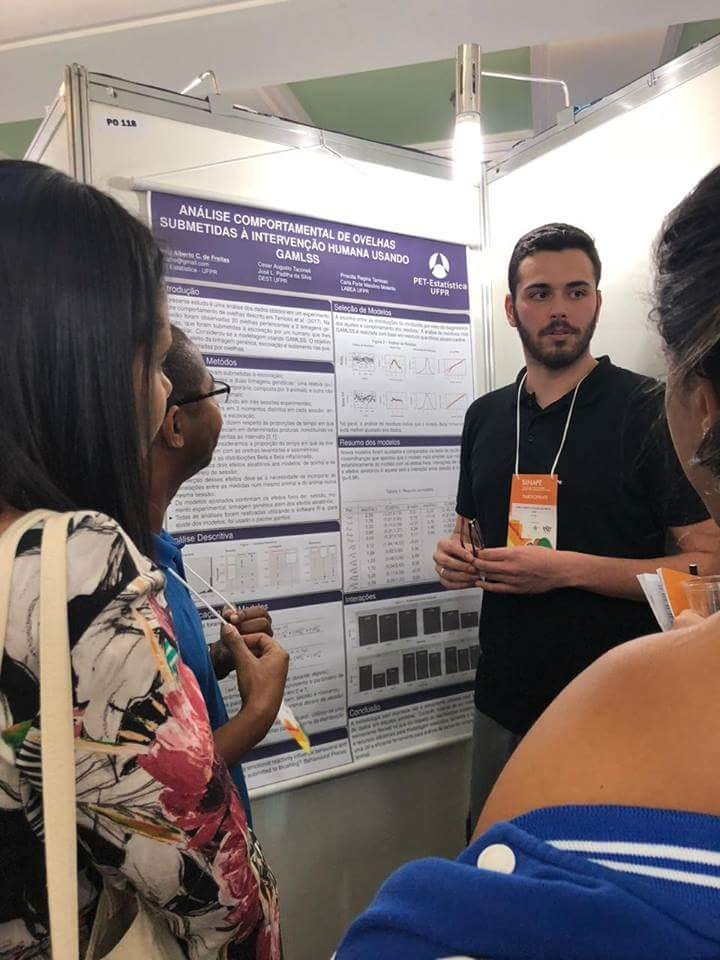
\includegraphics[height=6.5cm]{img/sinape4.jpg}
\end{center}

\end{frame}

% -----------------------------------------------------------------

\begin{frame}

\frametitle{SINAPE}

\begin{center}
  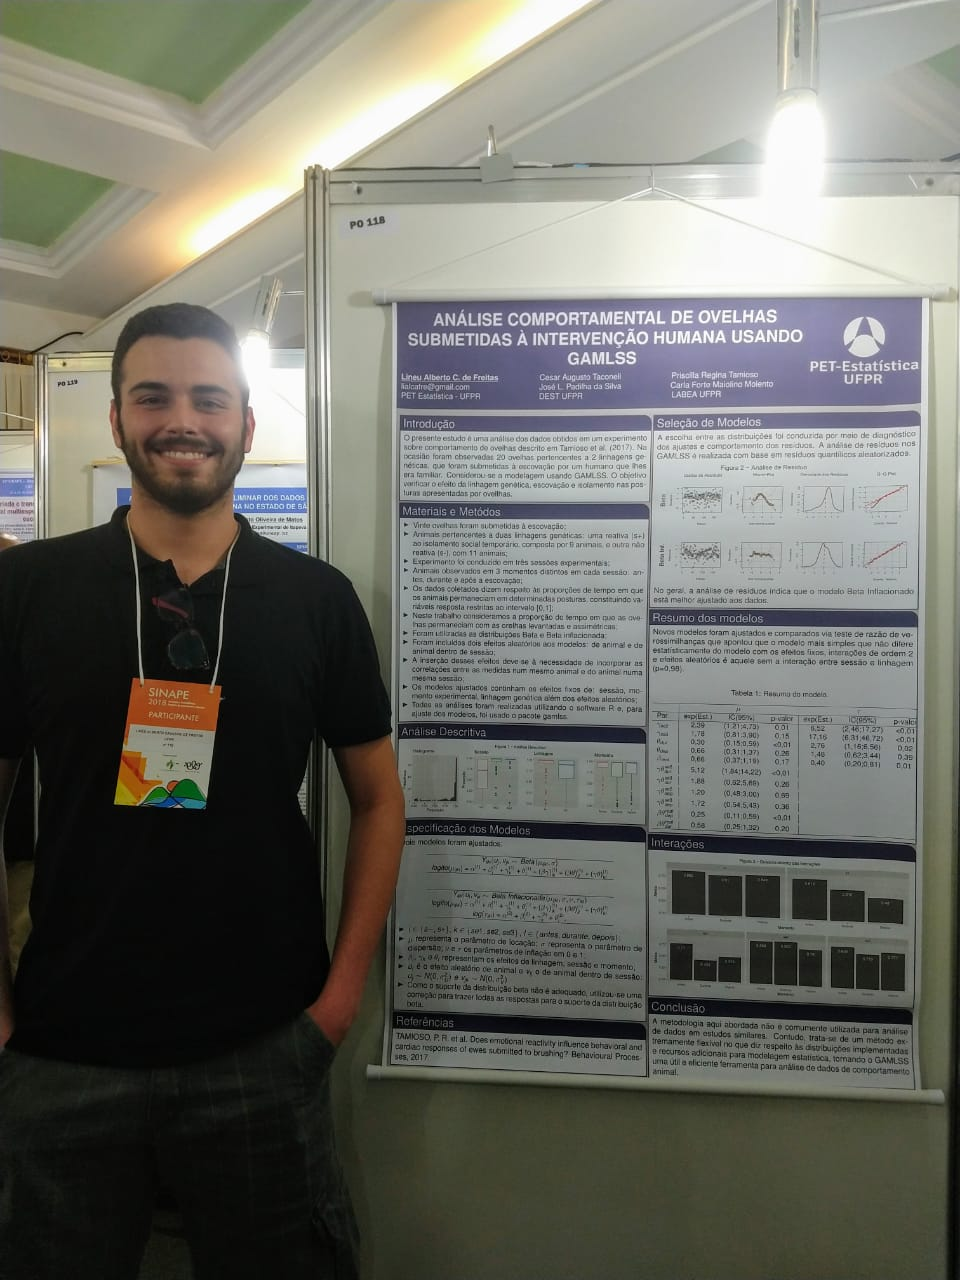
\includegraphics[height=6.5cm]{img/sinape2.jpg}
\end{center}

\end{frame}

% -----------------------------------------------------------------

\begin{frame}

\frametitle{SINAPE}

\begin{center}
  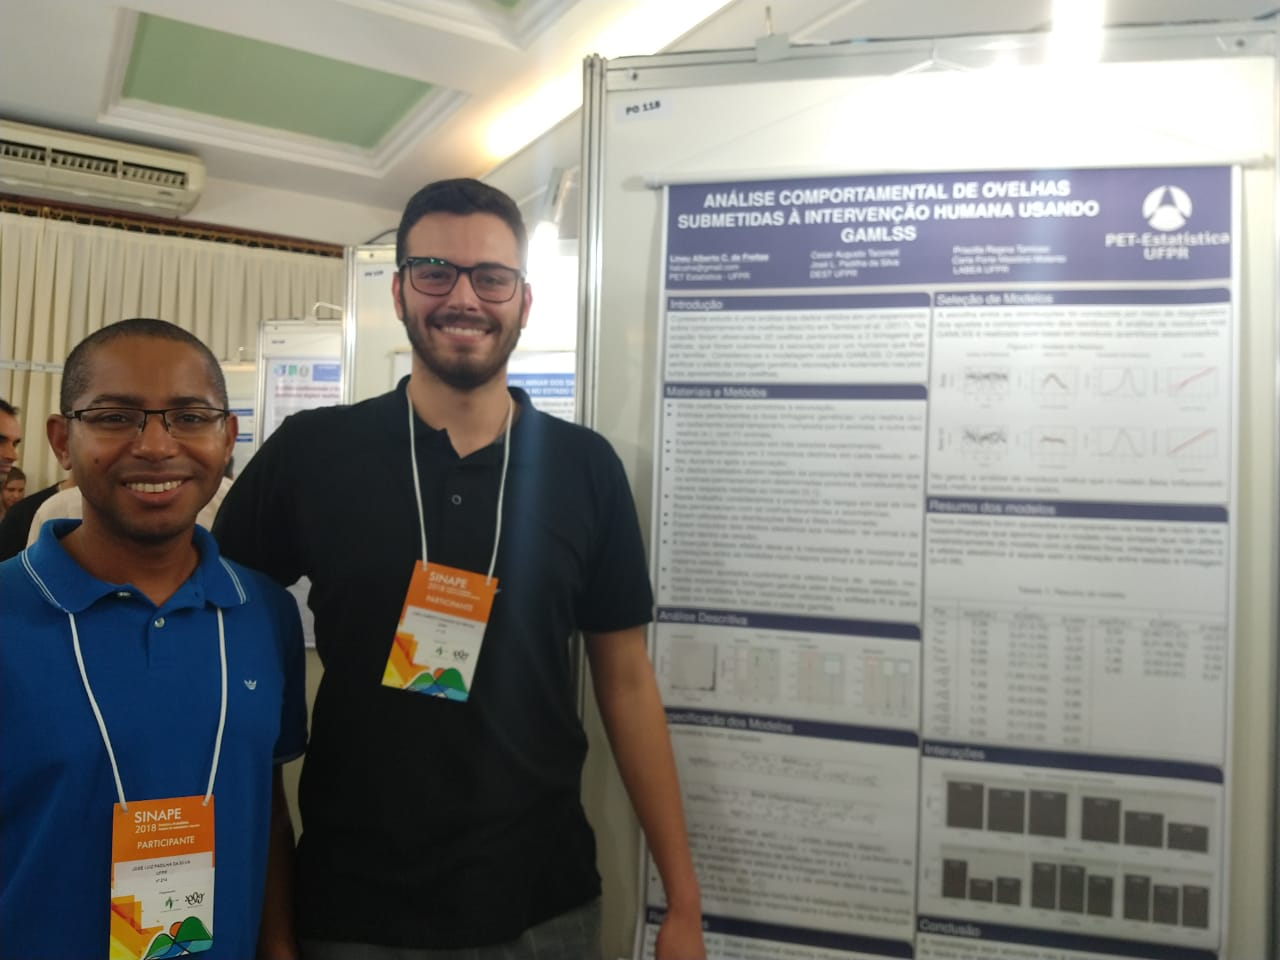
\includegraphics[height=6.5cm]{img/sinape3.jpg}
\end{center}

\end{frame}

% -----------------------------------------------------------------

\begin{frame}

\frametitle{SINAPE}

\begin{center}
  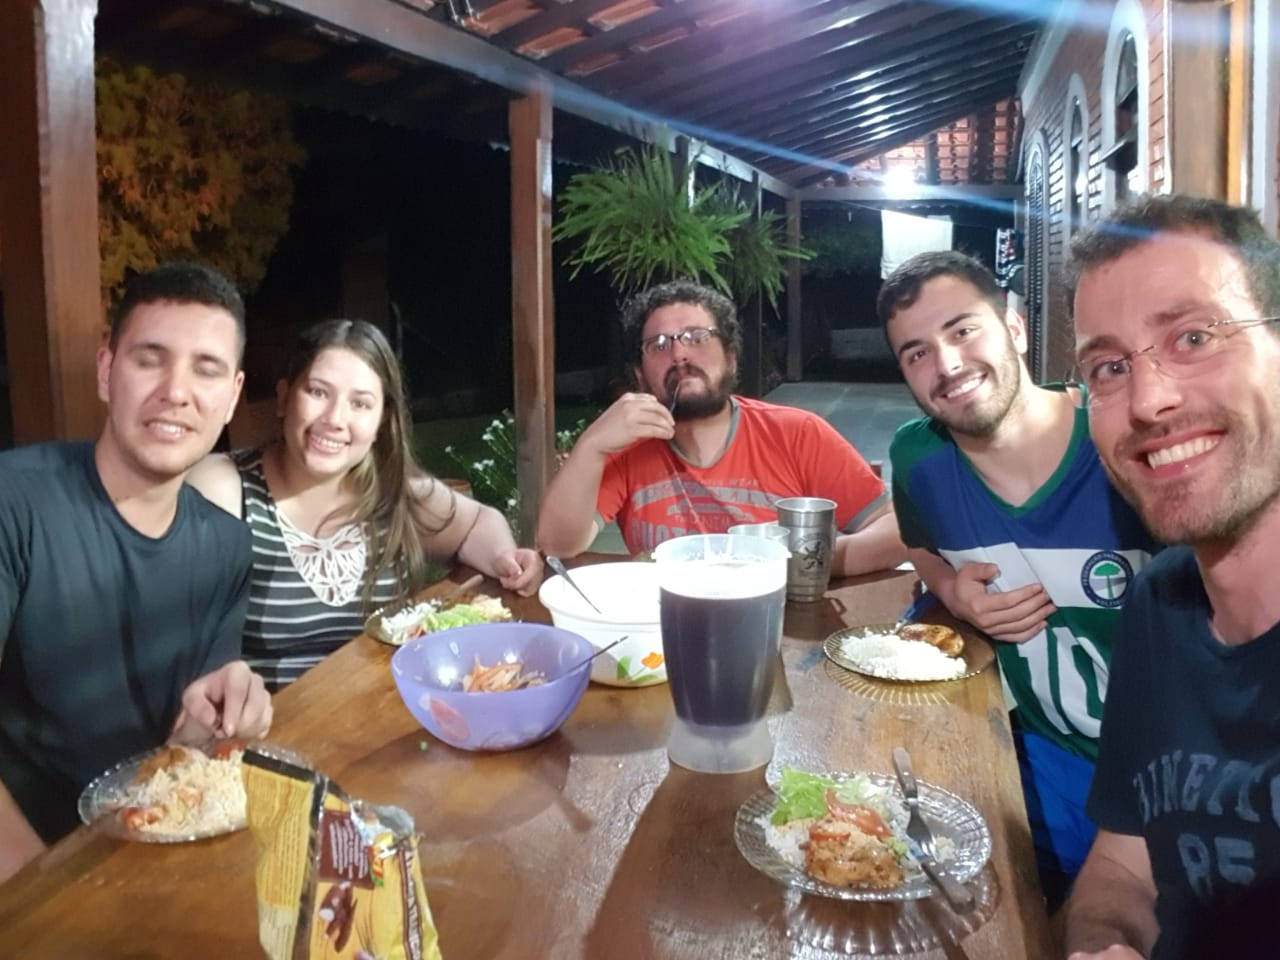
\includegraphics[height=6.5cm]{img/sinape1.jpg}
\end{center}

\end{frame}

% -----------------------------------------------------------------

\begin{frame}

\frametitle{SIEPE}

\begin{center}
  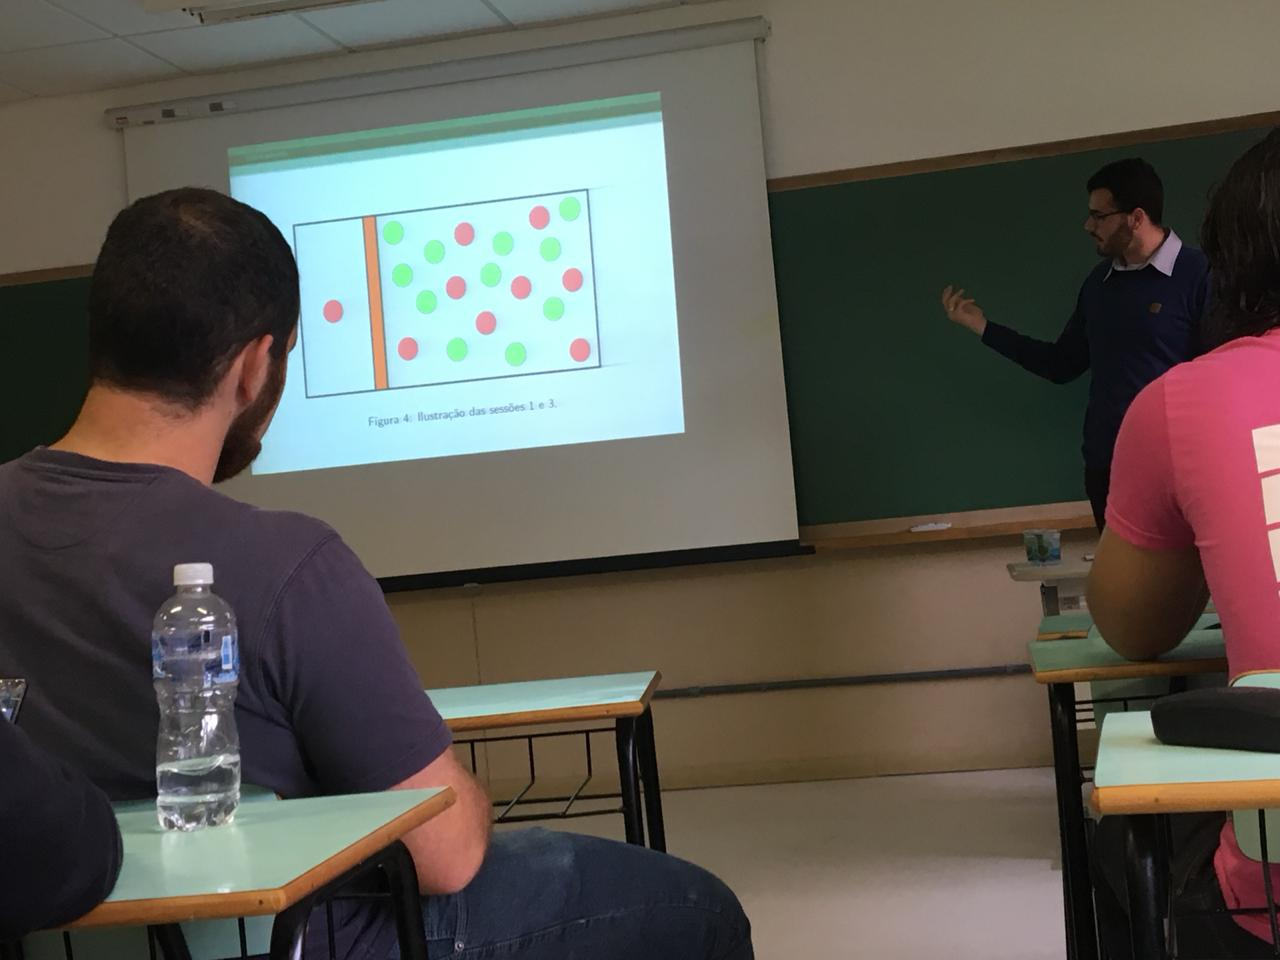
\includegraphics[height=6.5cm]{img/siepe1.jpg}
\end{center}

\end{frame}

% -----------------------------------------------------------------

\begin{frame}

\frametitle{Bradesco}

\begin{itemize}
  
  \itemsep 2ex
  
  \item Estágio no Departamento de Inteligência de Crédito Crédito do Banco Bradesco S.A.
  
  \item Portfólio de Produtos Parcelados com Garantia, Governança e Validação para Pessoa Física.
  
\end{itemize}

\begin{center}
  
\includegraphics[height=2cm]{img/bra.png}
\end{center}

\end{frame}

% -----------------------------------------------------------------

\begin{frame}

\frametitle{Vôlei UFPR}

\begin{center}
  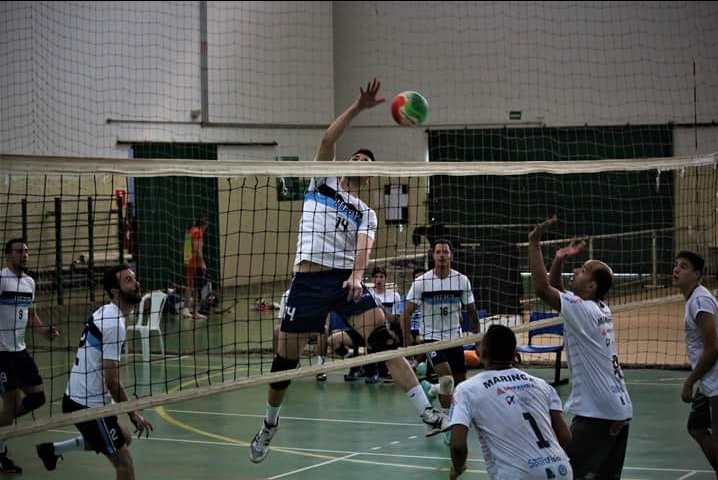
\includegraphics[height=6cm]{img/volei4.png}
\end{center}

\end{frame}

% -----------------------------------------------------------------

\begin{frame}

\frametitle{Vôlei UFPR}

\begin{center}
  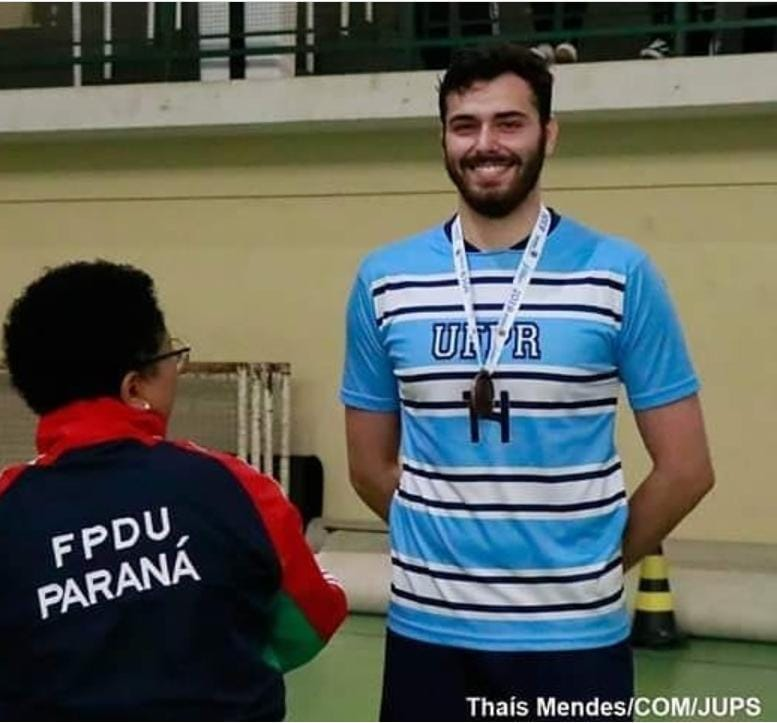
\includegraphics[height=6cm]{img/volei6.jpeg}
\end{center}

\end{frame}

% -----------------------------------------------------------------

\begin{frame}

\frametitle{Vôlei UFPR}

\begin{center}
  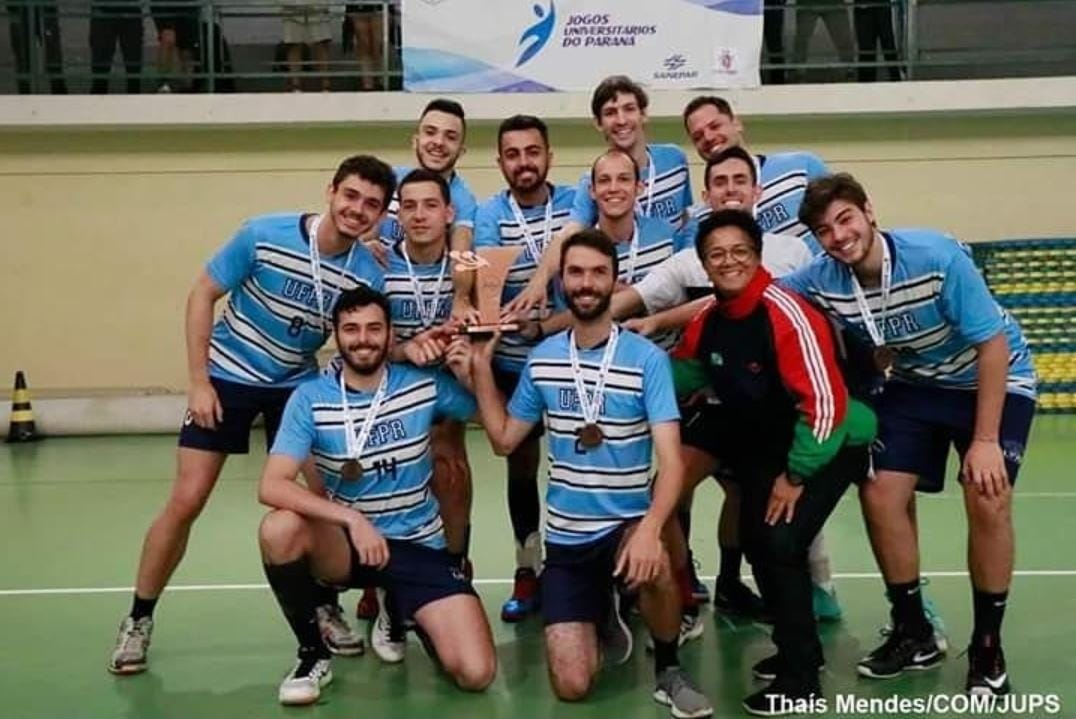
\includegraphics[height=6cm]{img/volei7.jpeg}
\end{center}

\end{frame}

% -----------------------------------------------------------------

\subsection{2019}

\begin{frame}[c, allowframebreaks]

\begin{center}

  {\huge \href{https://lineu96.github.io/st/}{2019}}
  
\end{center}

\end{frame}

% -----------------------------------------------------------------

\begin{frame}

\frametitle{Vôlei UFPR}

\begin{center}
  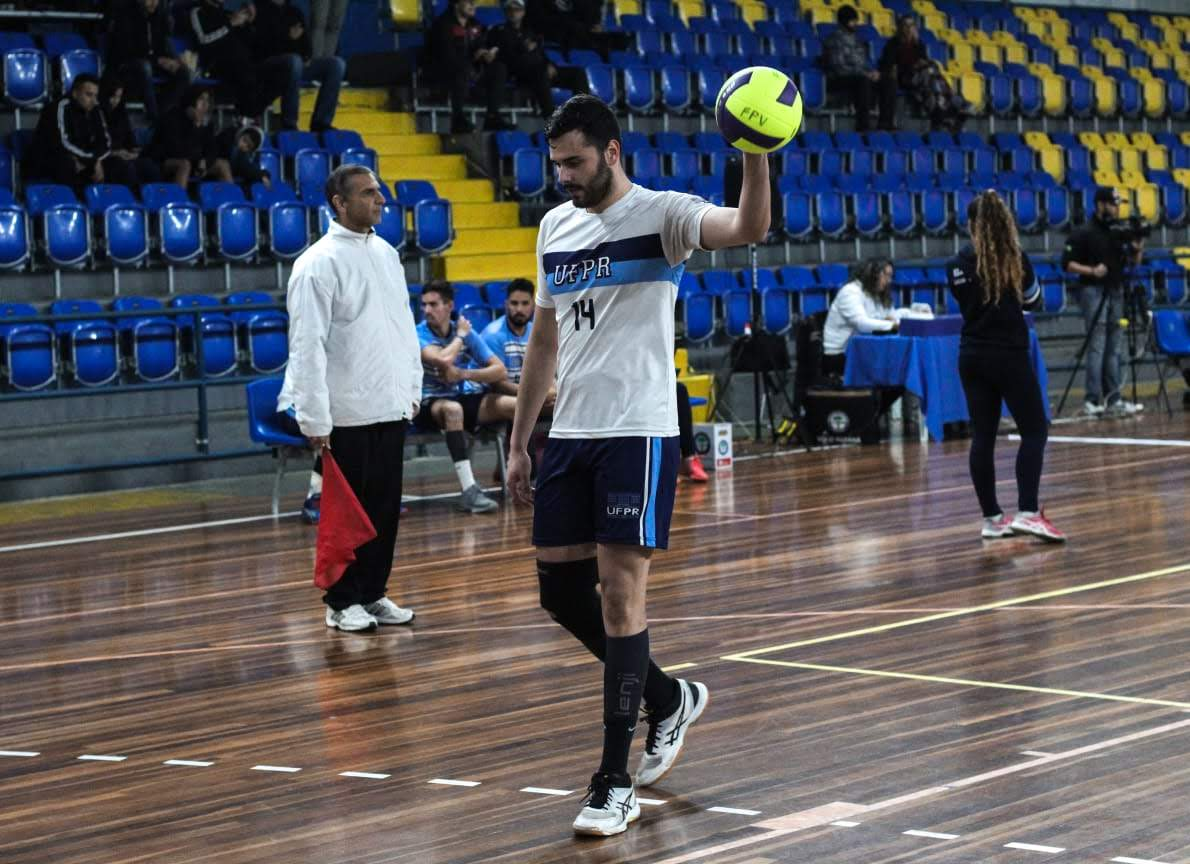
\includegraphics[height=6cm]{img/volei3.jpg}
\end{center}

\end{frame}

% -----------------------------------------------------------------

\begin{frame}

\frametitle{Vôlei UFPR}

\begin{center}
  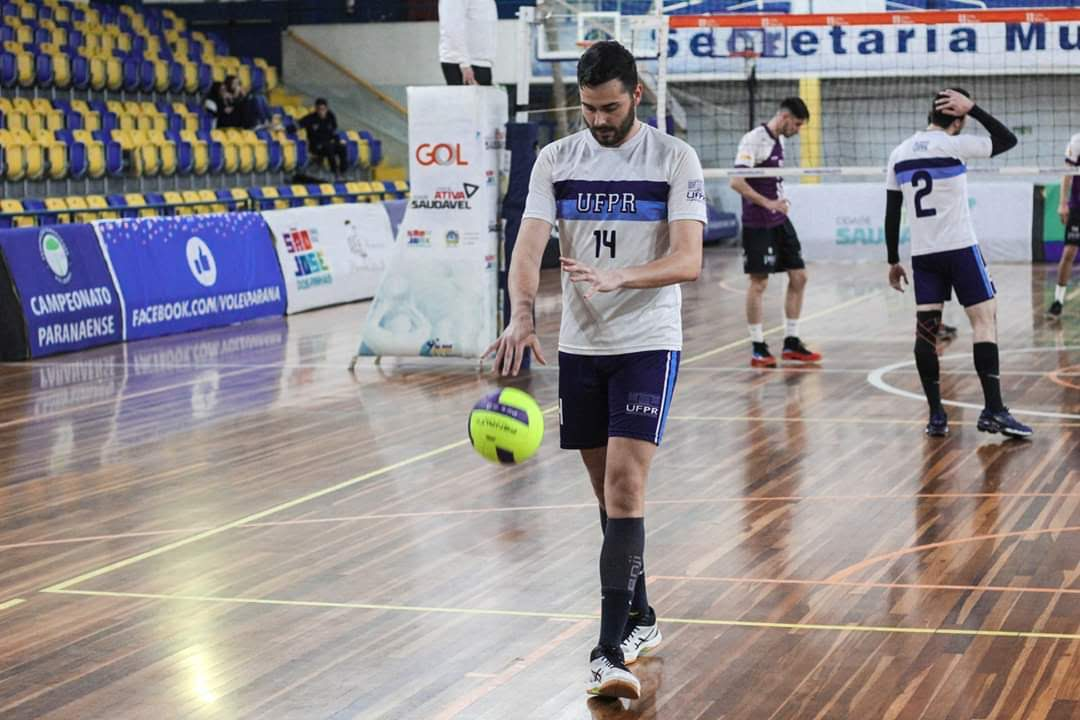
\includegraphics[height=6cm]{img/volei2.jpg}
\end{center}

\end{frame}

% -----------------------------------------------------------------

\begin{frame}

\frametitle{Vôlei UFPR}

\begin{center}
  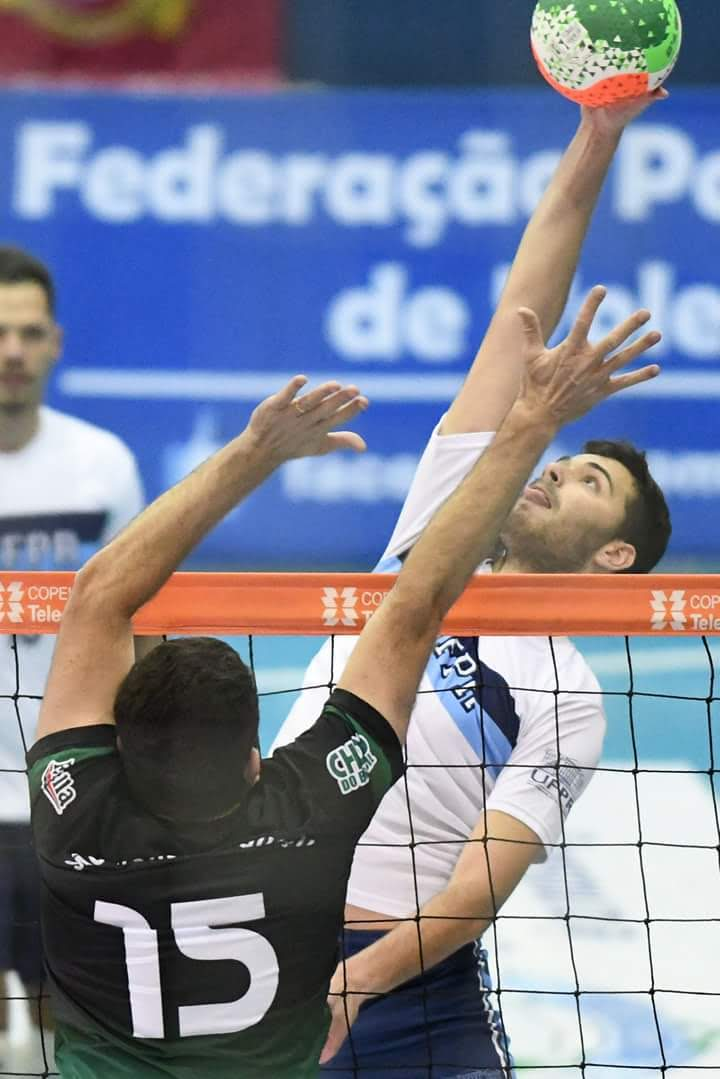
\includegraphics[height=6cm]{img/volei1.jpg}
\end{center}

\end{frame}

% -----------------------------------------------------------------


\begin{frame}

\frametitle{PET \& Bradesco}

\begin{center}
  
\includegraphics[height=3cm]{img/pet.png}\hspace{2em}
  
\includegraphics[height=4cm]{img/bradesco2.png}
\end{center}

\end{frame}

% -----------------------------------------------------------------


\begin{frame}

\frametitle{Minicurso R}

\begin{center}
  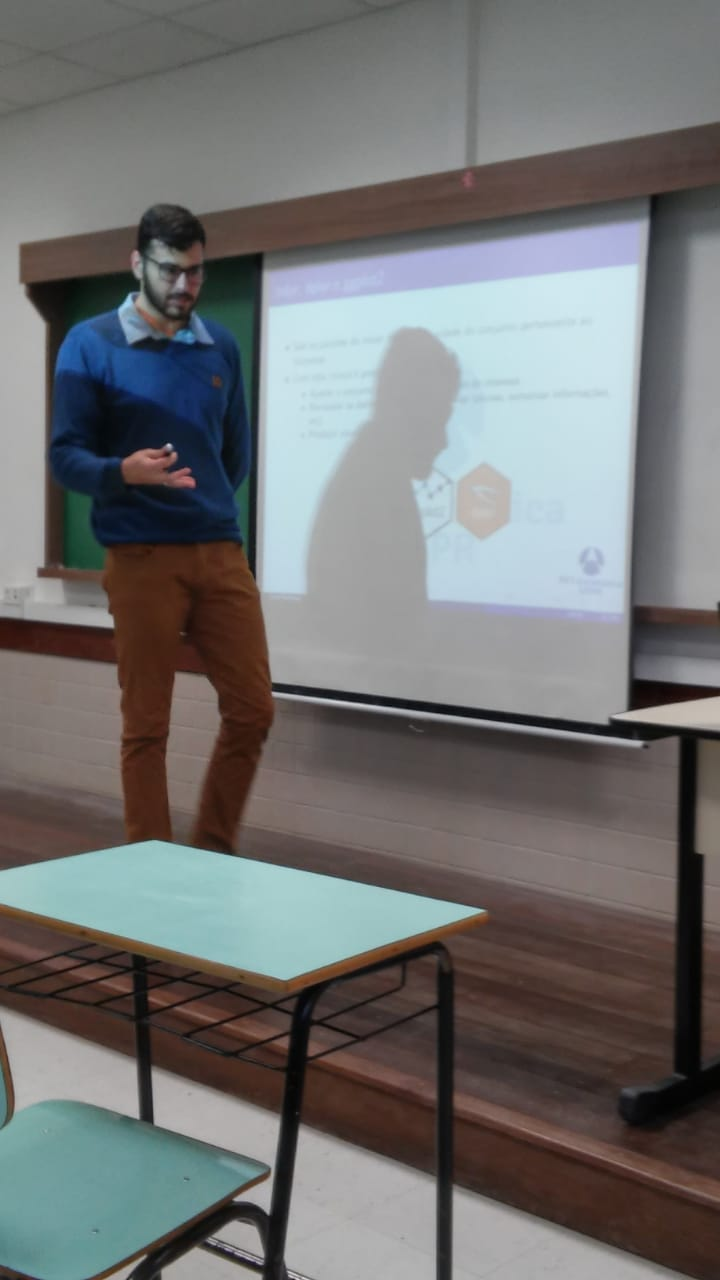
\includegraphics[height=6cm]{img/mincursor.jpg}\hspace{2em}
  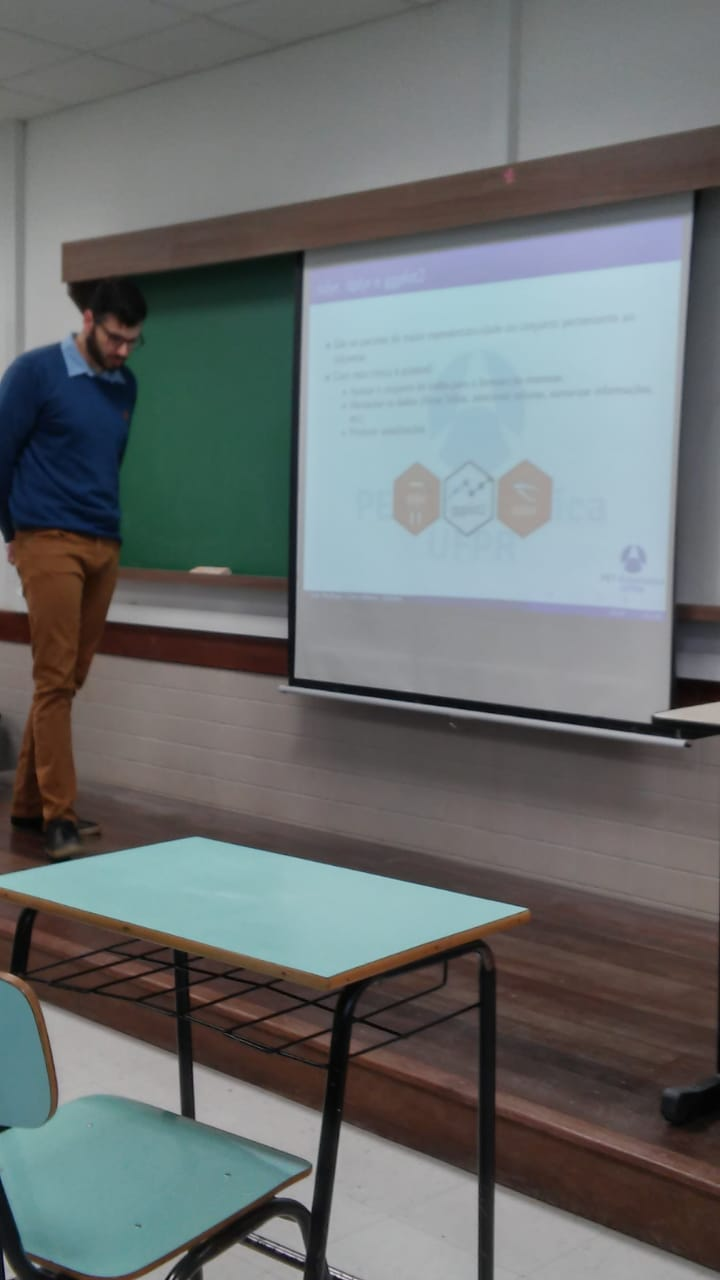
\includegraphics[height=6cm]{img/minicursor2.jpg}
\end{center}

\end{frame}

% -----------------------------------------------------------------

\begin{frame}

\frametitle{1ºE DSBD}

\begin{center}
  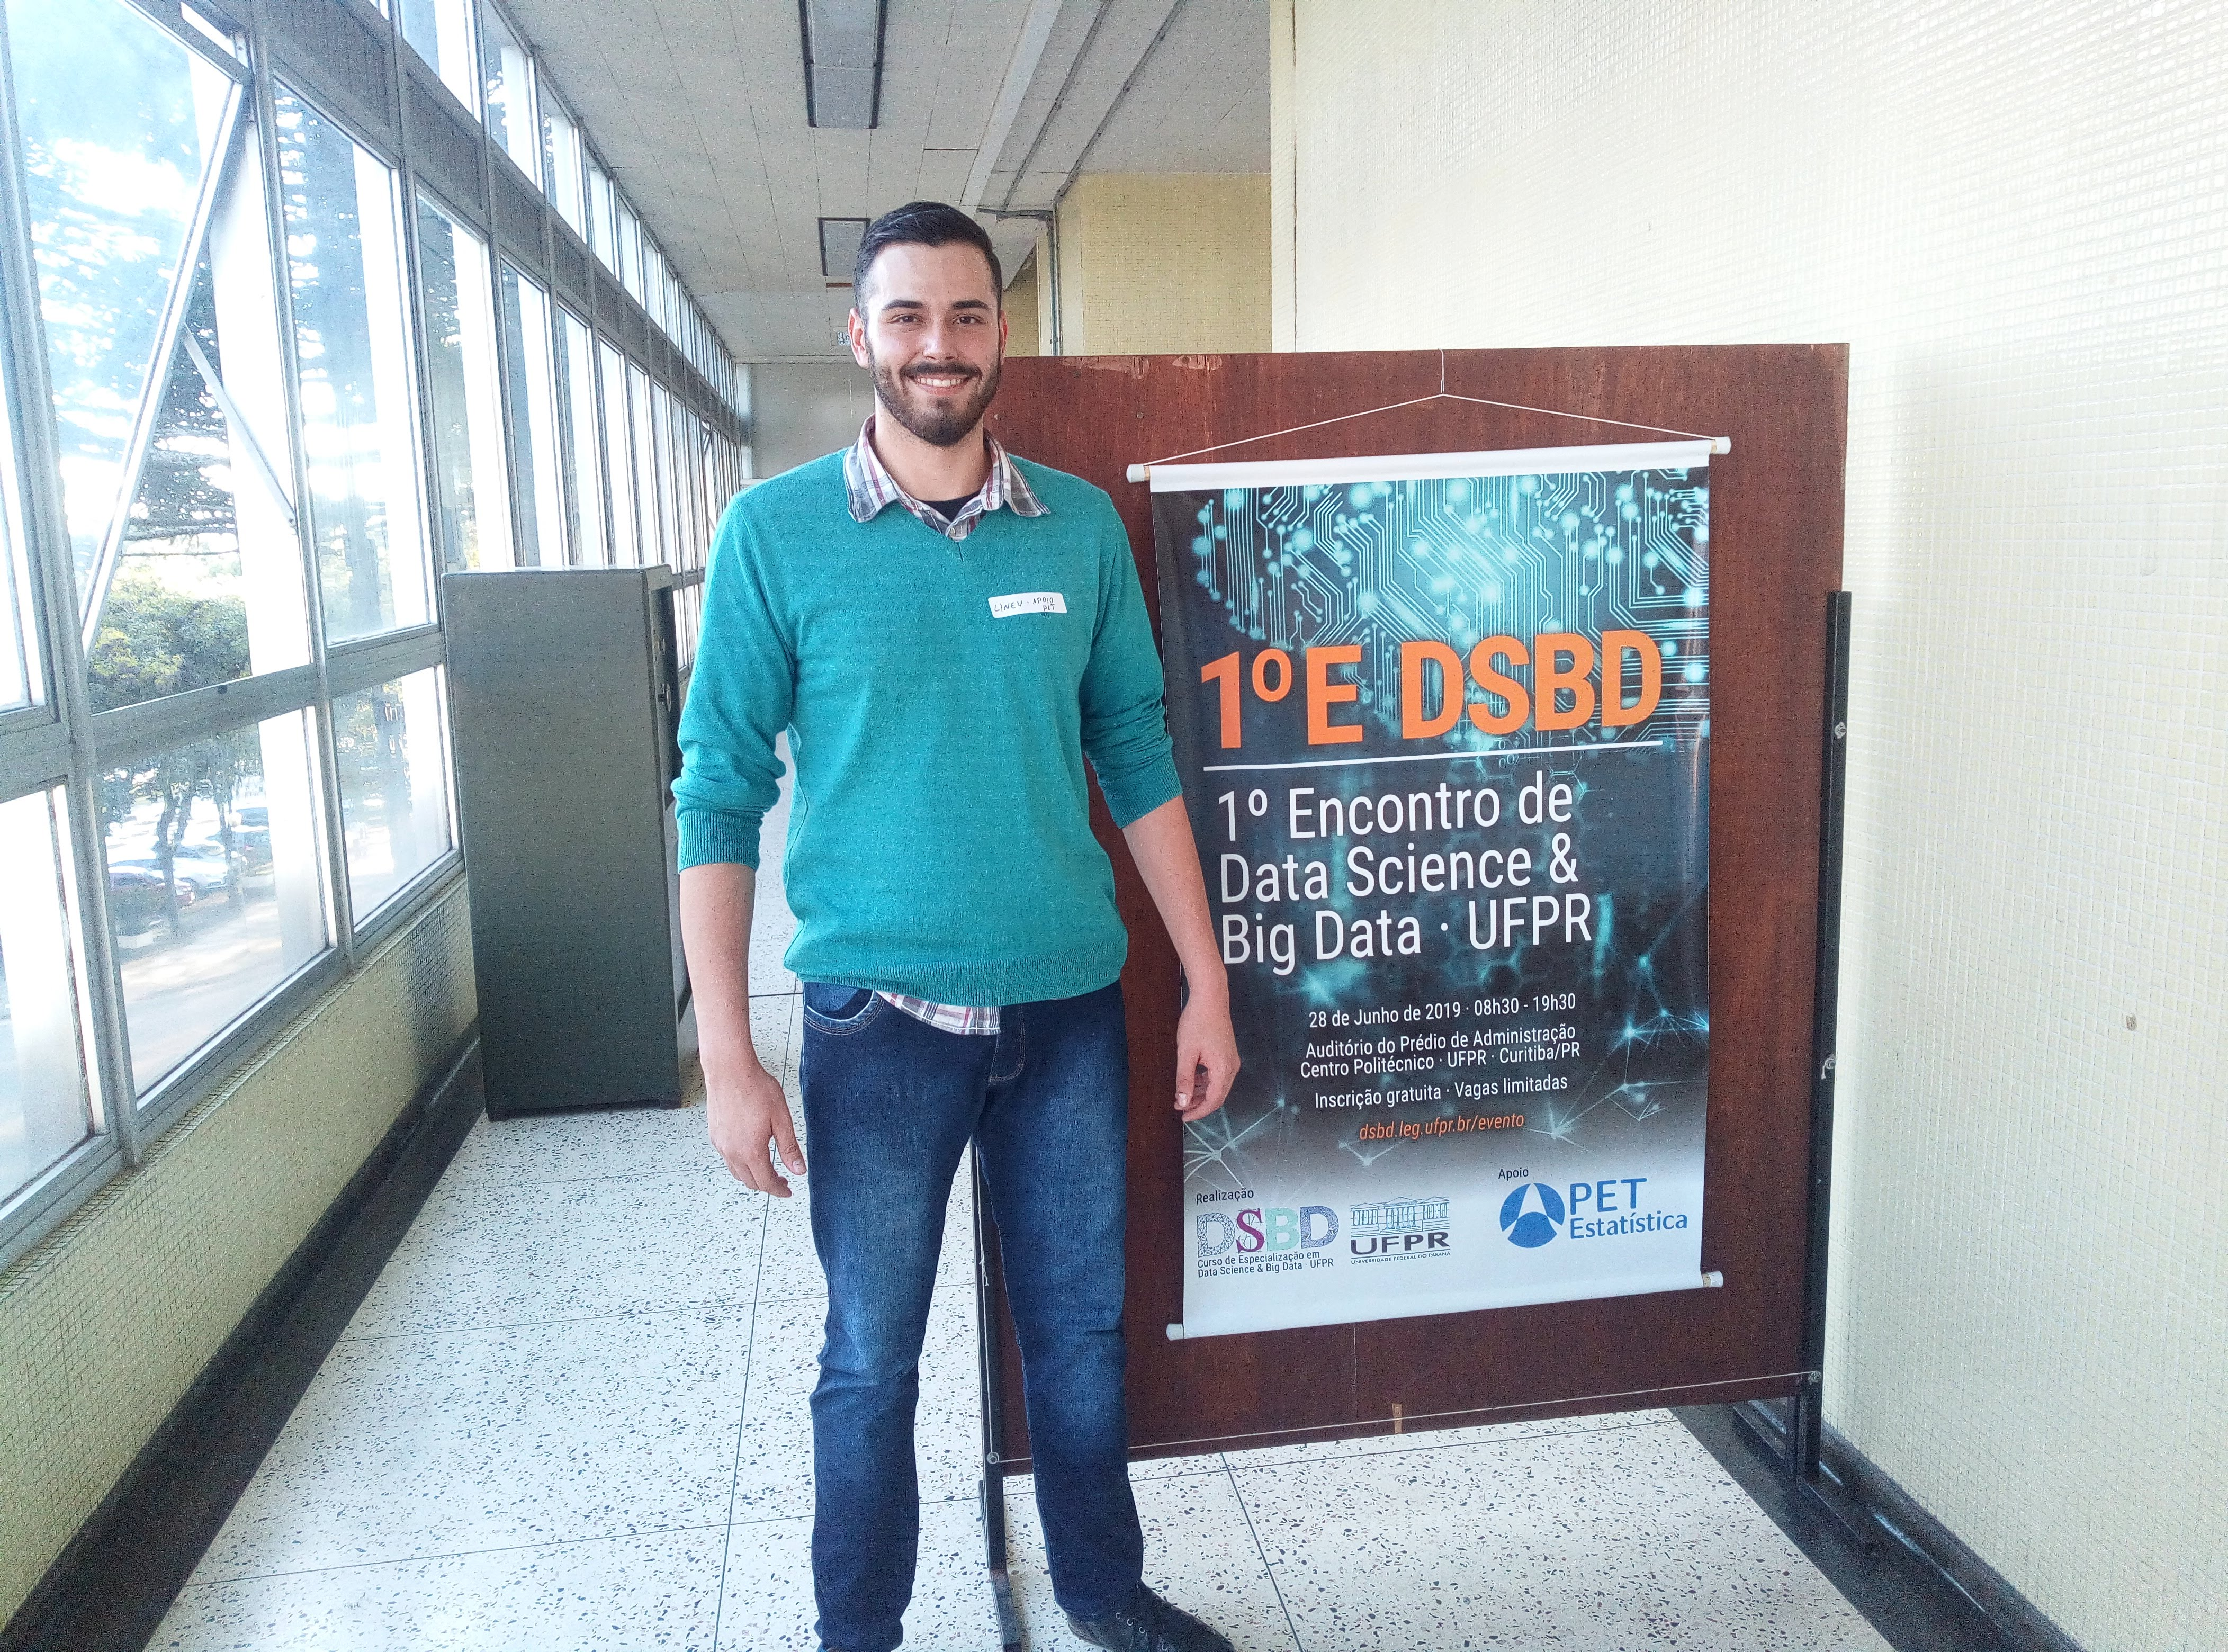
\includegraphics[height=6cm]{img/dsbd.jpg}
\end{center}

\end{frame}

% -----------------------------------------------------------------

\begin{frame}

\frametitle{TCC}

\begin{center}
  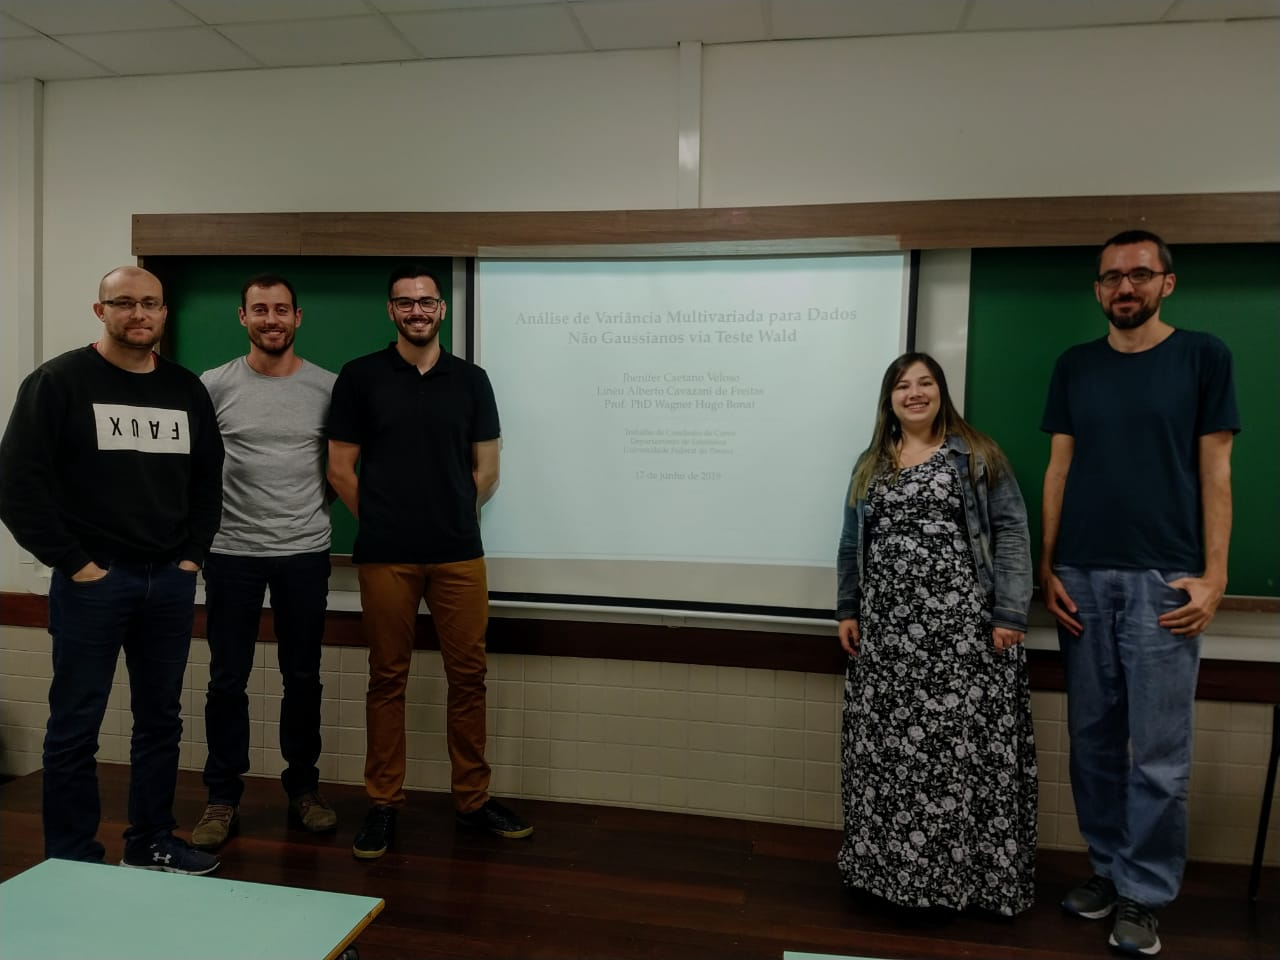
\includegraphics[height=6cm]{img/tcc.jpg}
\end{center}

\end{frame}

% -----------------------------------------------------------------

\subsection{2020}

\begin{frame}[c, allowframebreaks]

\begin{center}

  {\huge \href{https://lineu96.github.io/st/}{2020}}
  
\end{center}

\end{frame}

% -----------------------------------------------------------------

\begin{frame}

\frametitle{Mestrado}

\begin{center}
  
\includegraphics[height=3cm]{img/unicamp.jpeg}\hspace{2em}
  \includegraphics[height=3cm]{img/imecc.png}
\end{center}

\end{frame}

% -----------------------------------------------------------------

\begin{frame}

\frametitle{Mestrado}

\begin{center}
  \includegraphics[height=6cm]{img/unicamp_aprova.png}
\end{center}

\end{frame}

% -----------------------------------------------------------------

\begin{frame}

\frametitle{Mestrado}

\begin{center}
  \includegraphics[height=6cm]{img/lncc.png}
\end{center}

\end{frame}

% -----------------------------------------------------------------

\begin{frame}

\frametitle{Mestrado}

\begin{center}
  \includegraphics[height=2cm]{img/ufpr-transparent.png}\hspace{2em}
  \includegraphics[height=2cm]{img/dsbd-2x2-trans.png}
\end{center}

\end{frame}

% -----------------------------------------------------------------

\begin{frame}

\frametitle{Mestrado}

\begin{center}
  \includegraphics[height=5cm]{img/mestrado.png}
\end{center}

\end{frame}

% -----------------------------------------------------------------

\begin{frame}

\frametitle{Mestrado}

\begin{center}
  \includegraphics[height=1.8cm]{img/capes_tp2.png}\hspace{2em}
  \includegraphics[height=1.8cm]{img/ufpr-transparent.png}\hspace{2em}
  \includegraphics[height=1.8cm]{img/dsbd-2x2-trans.png}
\end{center}

\end{frame}


% -----------------------------------------------------------------

\begin{frame}

\frametitle{MEPC}

\begin{center}
  \includegraphics[height=6cm]{img/mepc.jpg}
\end{center}

\end{frame}

% -----------------------------------------------------------------

\begin{frame}

\frametitle{PET Convida}

\begin{center}
  \includegraphics[height=6cm]{img/petcv.jpeg}
\end{center}

\end{frame}

% -----------------------------------------------------------------

\subsection{2021}

\begin{frame}[c, allowframebreaks]

\begin{center}

  {\huge \href{https://lineu96.github.io/st/}{2021}}
  
\end{center}

\end{frame}


% -----------------------------------------------------------------

\begin{frame}

\frametitle{Artigo}

\begin{center}
  \includegraphics[height=6cm]{img/paper.png}
\end{center}

\end{frame}


% -----------------------------------------------------------------

\begin{frame}

\frametitle{MEPC}

\begin{center}
  \includegraphics[height=6cm]{img/mepc.jpg}
\end{center}

\end{frame}

% -----------------------------------------------------------------

\begin{frame}

\frametitle{MEPC}

\begin{center}
  \includegraphics[height=6cm]{img/mepc2.png}
\end{center}

\end{frame}

% -----------------------------------------------------------------

\section{Atividades realizadas}

\begin{frame}

\frametitle{Resumo das atividades}

  \begin{itemize}
  
    \itemsep 1ex
  
  \item Eventos. 
  
  \item Estágios não obrigatórios.
  
  \item PET.
  
  \item Monitoria.
  
  \item Minicursos e aulas particulares.
  
  \item Esporte.
  
  \item Projetos de pesquisa.
  
  \item Mestrado (em andamento).

  \end{itemize}
\end{frame}

% -----------------------------------------------------------------

\section{Meus conselhos e percepções}

\begin{frame}

\frametitle{Resumo das atividades}

  \begin{itemize}
  
    \itemsep 2ex
  
  \item Não é curso fácil.

  \item O curso de graduação em Estatística da UFPR é um dos melhores do Brasil.

  \item Vários professores são reconhecidos nacional e internacionalmente.

  \item Estágios são atrativos (\$\$), mas tomem cuidado.

  \item Se vocês tiverem condições, aproveitem as oportunidades acadêmicas. 
  

  \end{itemize}
\end{frame}

% -----------------------------------------------------------------

\begin{frame}[c, allowframebreaks]

\begin{center}

  {\huge \href{https://lineu96.github.io/st/}{Obrigado!}}
  
  \vspace{0.5cm}
    
  {\normalsize \href{https://lineu96.github.io/st/}{Lineu Alberto Cavazani de Freitas}}
  
  {\normalsize \href{https://lineu96.github.io/st/}{lineuacf@gmail.com}}
  
  {\normalsize \href{https://lineu96.github.io/st/}{https://lineu96.github.io/st/}}
  
  {\normalsize \href{http://www.prppg.ufpr.br/ppginformatica/?lang=pb}{PPG Informática}}


\begin{figure} % Inicia o ambiente de figuras
  %\subfigure{ % Começa a incluir a figura fig1.pdf
  %  \includegraphics[width=2cm]{img/logo.png}
  %} % Termina de incluir a figura fig1.pdf
  \subfigure{ % Começa a incluir a figura fig2.pdf na mesma linha da figura fig1.pdf
    \includegraphics[width=3cm]{img/ufpr-transparent.png}
  } % Termina de incluir a figura fig2.pdf
  %\subfigure{ % Começa a incluir a figura fig3.pdf na linha abaixo
  %  \includegraphics[width=1.4cm]{img/dsbd-2x2-trans.png}
  %} % Termina de incluir a figura fig3.pdf
\end{figure} % Fecha o ambiente de figuras

\end{center}

\end{frame}

\end{document}
